

To meet the wide-ranging goals expected by the LHC physics program, the CMS detector \cite{CMSTDR} was installed at insertion point 5 (P5) along the LHC ring, and records the proton-proton collisions delivered by the LHC. The distinguishing feature of the CMS detector is a powerful superconducting solenoid magnet. Hermetic in coverage and cylindrical in geometry, the CMS detector is divided into three subsystems: the inner tracker, the hadronic and electromagnetic calorimeters, and the muon system. A two-level trigger system is responsible for rejecting uninteresting physics events to reduce the storage size of the collision data. A diagram of the CMS detector is shown in Fig.~\ref{fig:CMSDiagram}.

\begin{figure}[H]
    \centering
    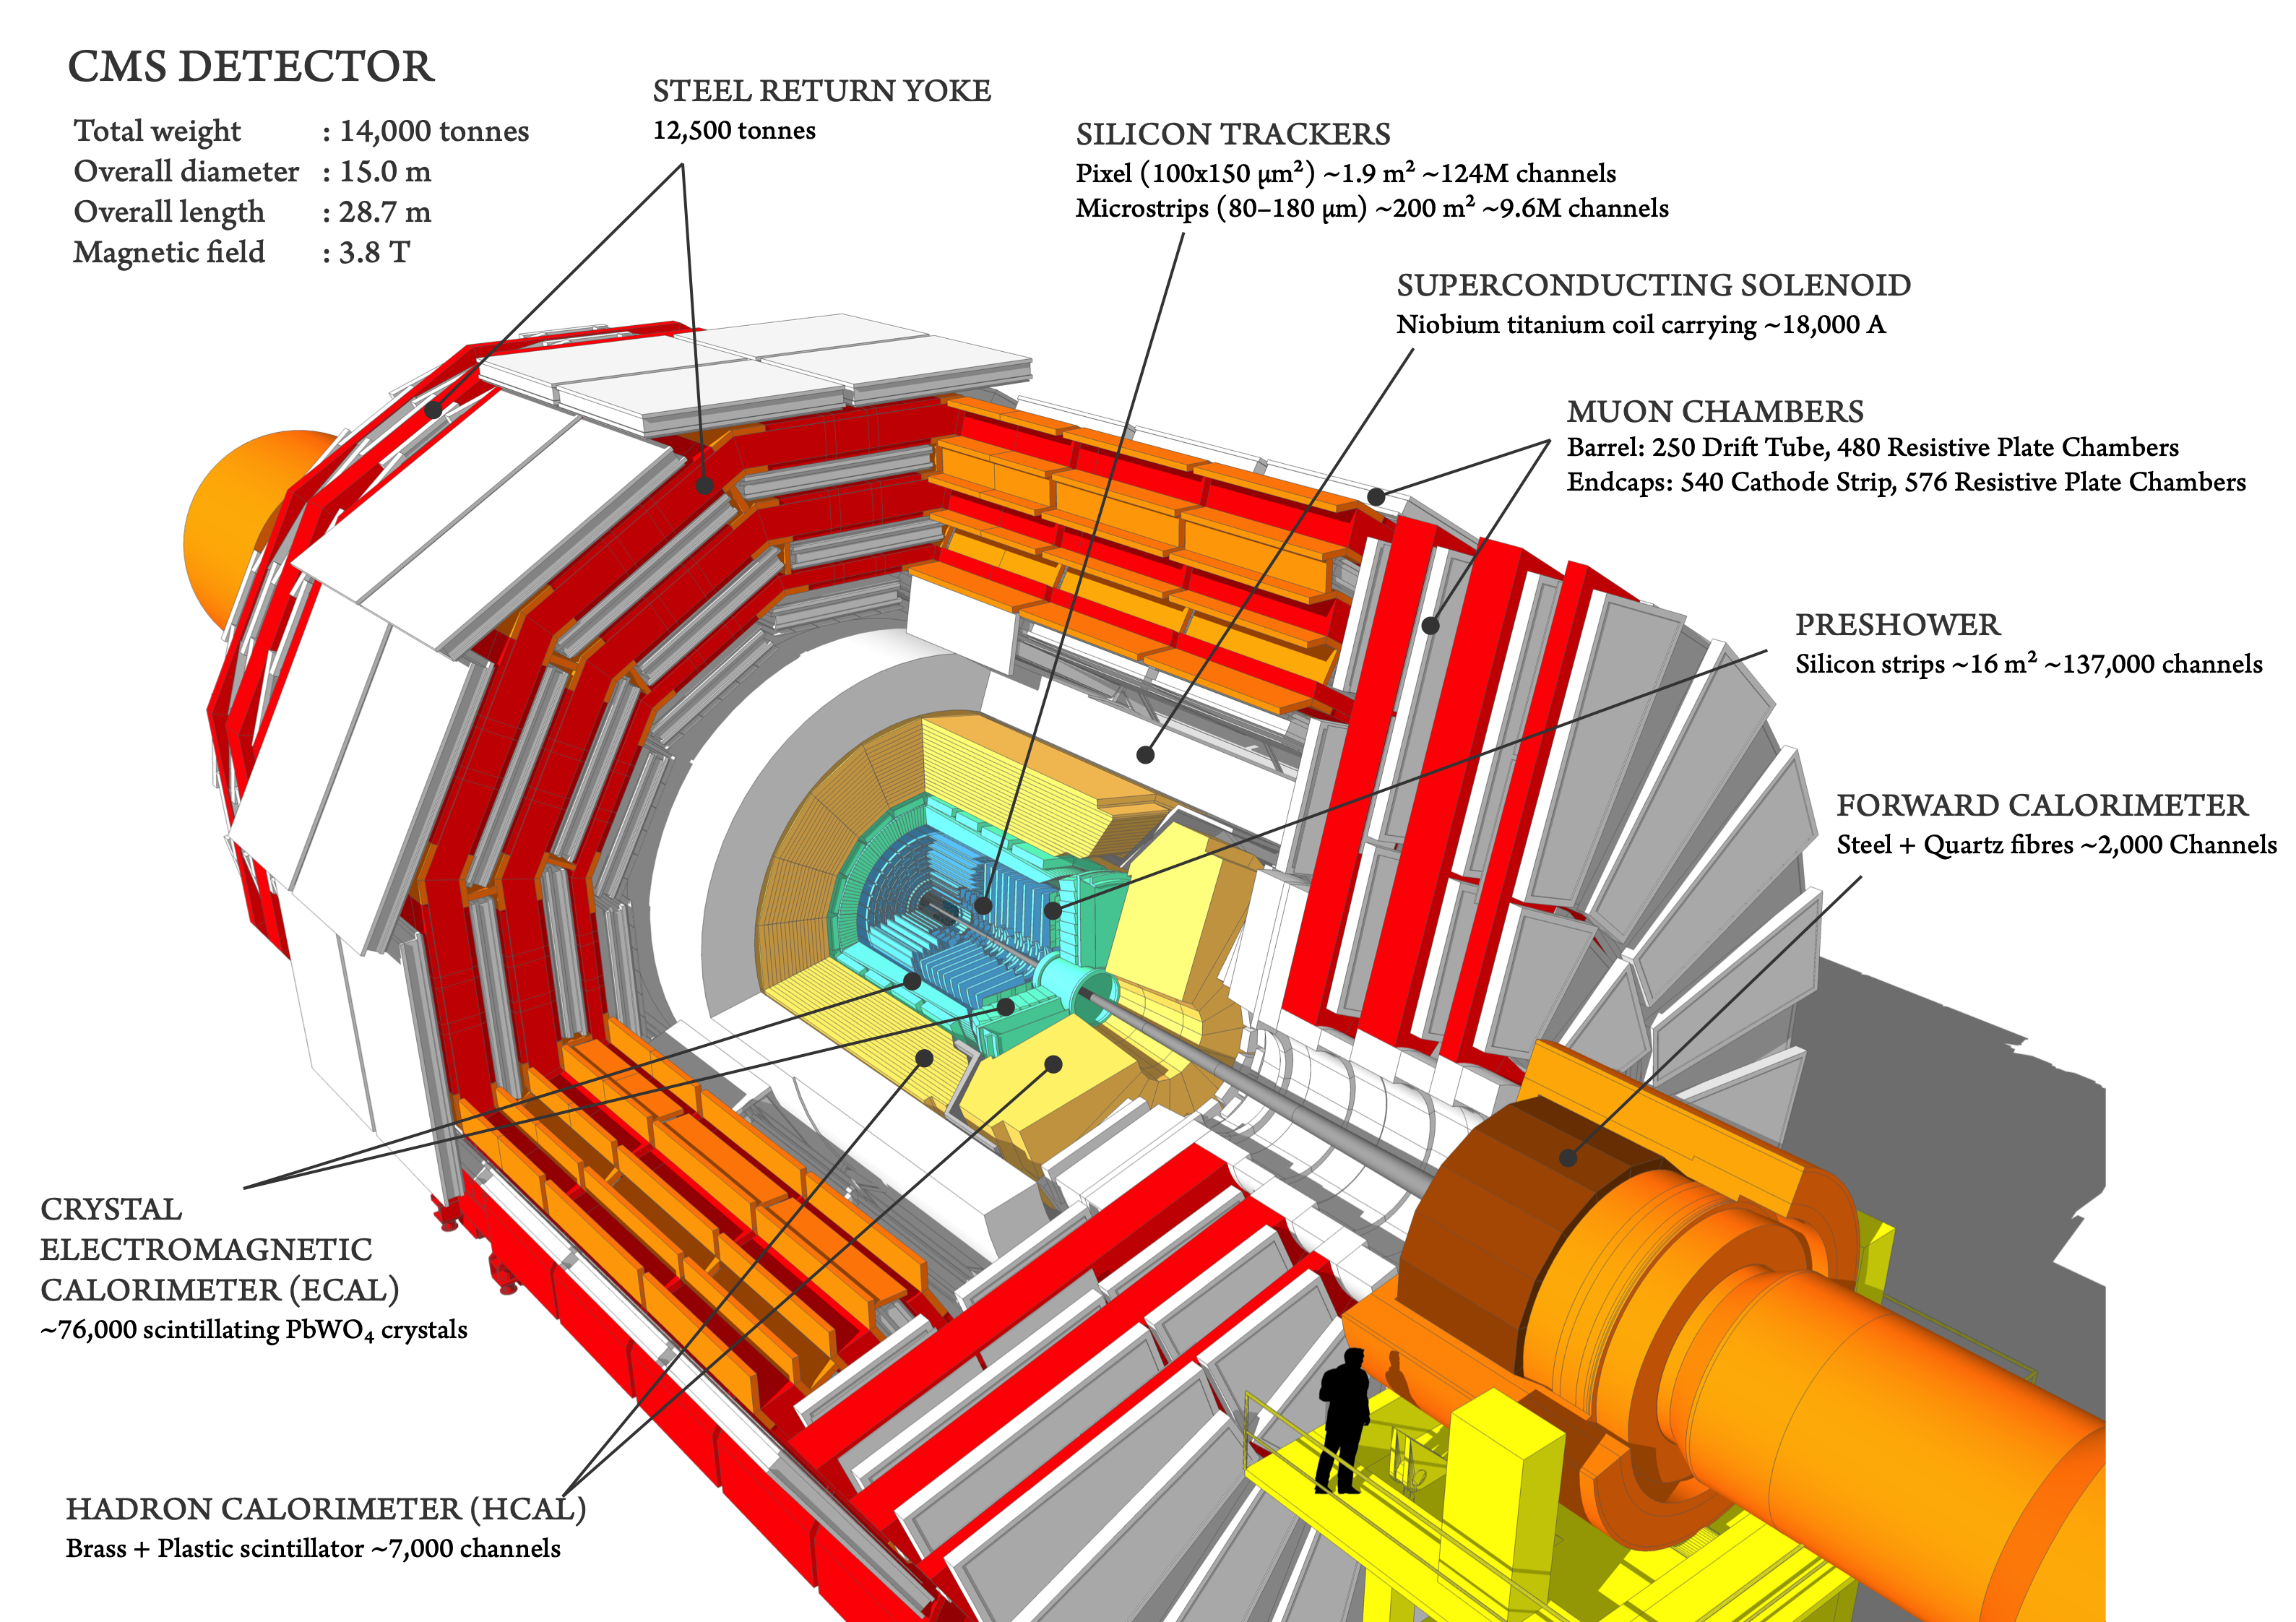
\includegraphics[width=1\textwidth]{Images/CMS/CMSDiagram.png}
    \caption{A cutaway diagram of the CMS detector}
    \label{fig:CMSDiagram}
\end{figure}

Data-taking periods at LHC experiments are grouped into runs each lasting several years, separated by long shutdowns (LS) where important upgrades to the detectors are made. Run 1 saw CMS begin data-taking in 2010 with the recording of collisions at $\sqrt{s}=\SI{7}{TeV}$, co-discovering the Higgs boson in 2012, before ramping down in 2013 for two years of upgrades in LS1. In 2015, CMS started recording $\sqrt{s}=\SI{13}{TeV}$ collisions for Run 2 of data-taking which lasted until 2018. Following Run 2, more upgrades to the detector were made, and in 2022 CMS launched Run 3 of data-taking, which remains ongoing.


\subsection{Tracker} \label{sec:InnerTracker}

The inner-most detector, closest to the beam pipe, is the CMS tracker system, which uses two technologies: silicon pixels and silicon microstrips (photos of each shown in Fig.~\ref{fig:Tracker}). The purpose of the CMS tracking system is to reconstruct the trajectories of electromagnetically charged physics objects close to the interaction point and measure the positions of the primary vertex (PV) of collisions and secondary vertecies of displaced decays (e.g., B hadrons). Owing to its proximity to the primary-interaction point, the CMS tracker is subject to the highest dosage radiation of all the subsystems.

\begin{figure}[H]
    \centering
    \resizebox{1\textwidth}{!}{
    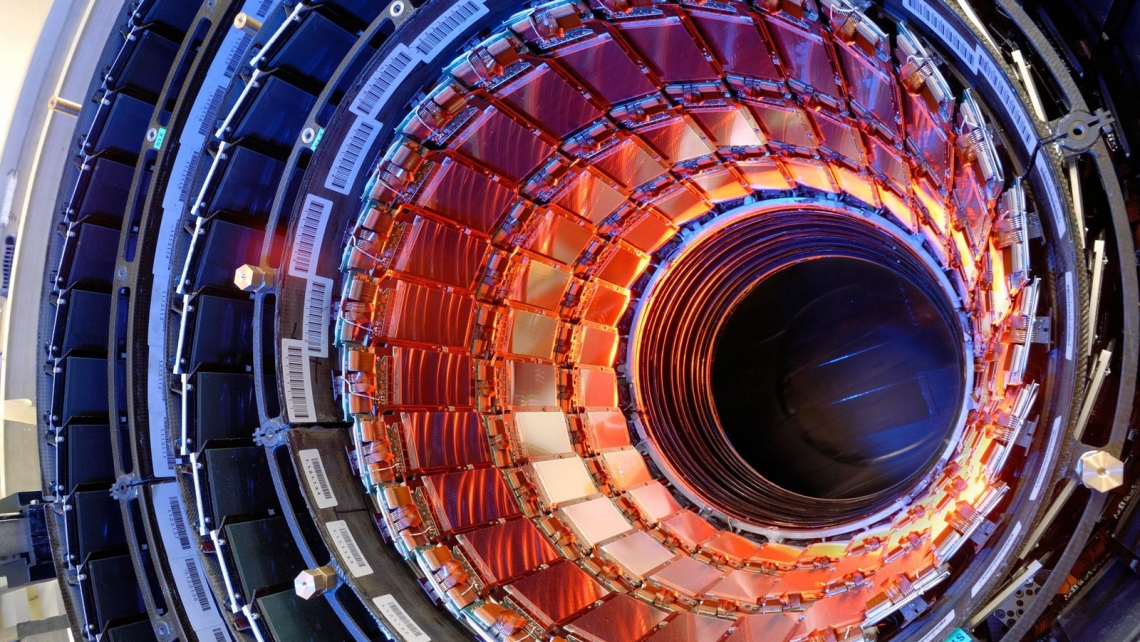
\includegraphics[height=\textwidth]{Images/CMS/SiStripTracker.jpg}
    \quad
    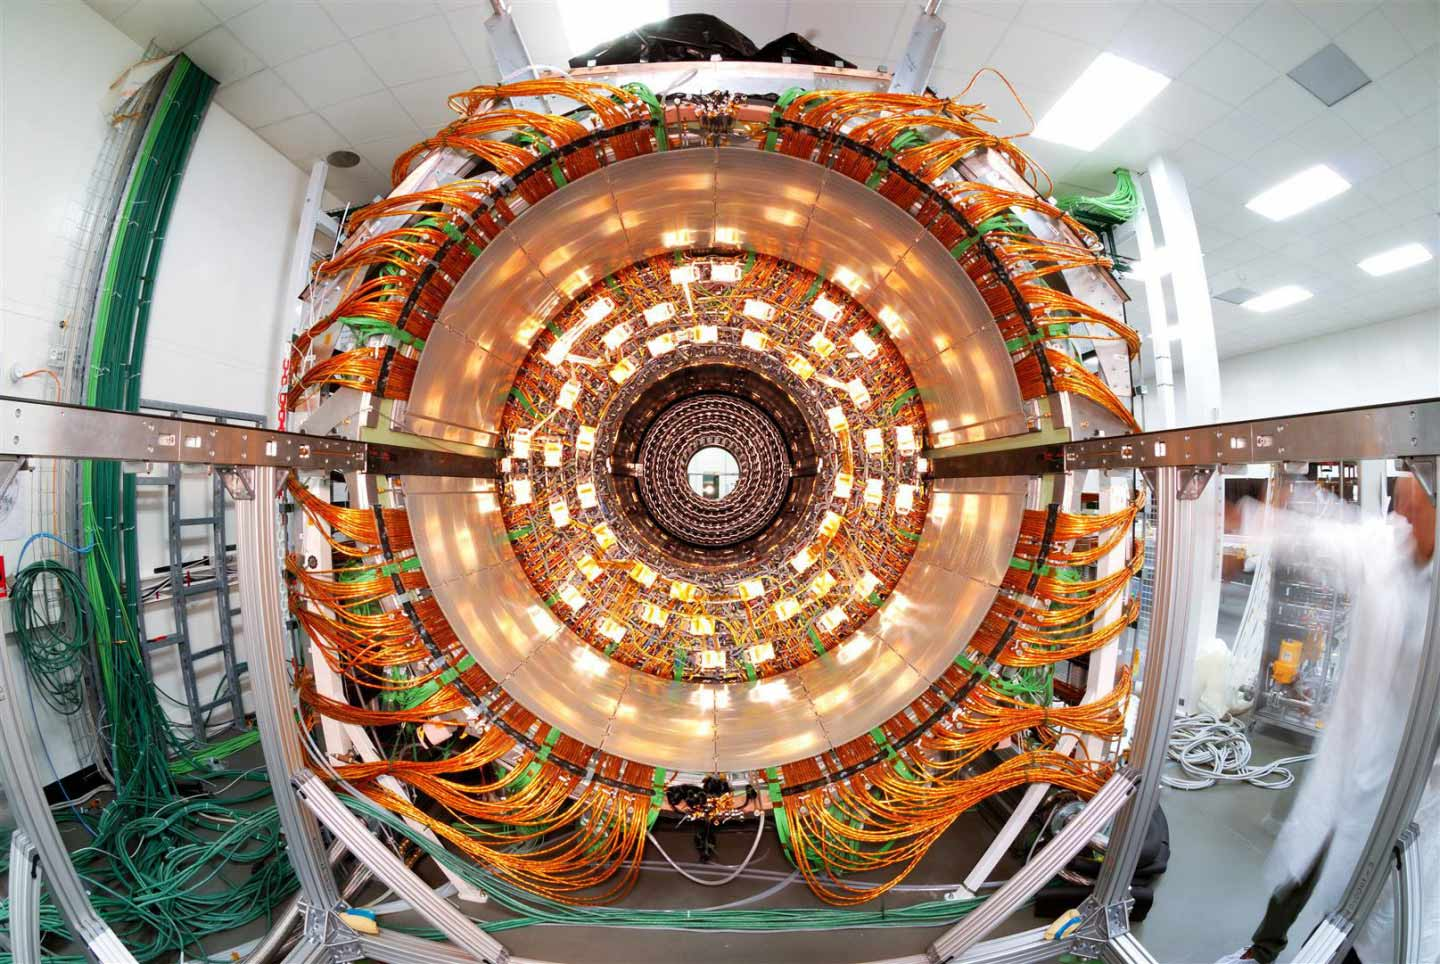
\includegraphics[height=\textwidth]{Images/CMS/PixelTracker.jpg}
    } 
    \caption{Photographs of the silicon strip detectors (left) and the pixel detectors (right) in the tracker barrel prior to installation.}
    \label{fig:Tracker}
\end{figure}

\subsubsection{Pixel tracker} \label{sec:PixelTracker}

The silicon pixel detector, upgraded to the Phase-1 pixel detector \cite{PixelUpgrade} during the 2016-2017 year-end technical stop of Run 2 to cope with higher integrated luminosities, provides a four-hit coverage in the pseudorapidity range $|\eta|<2.5$. This is accomplished through silicon sensor modules, where each module is a $160\times 416$ pixel sensor connected to 16 readout chips. The modules are arranged in two configurations: four concentric barrel pixel detectors (BPIX) with 1,184 modules, and three endcap disk pixel detectors in the forward regions (FPIX) with 672 modules, for a total of 1856 silicon sensor modules and 124 million readout channels. A schematic of the upgraded Phase-1 pixel detector is provided in Fig.~\ref{fig:PixelDiagram} showing the pseudorapidity coverage.

\begin{figure}[H]
    \centering
    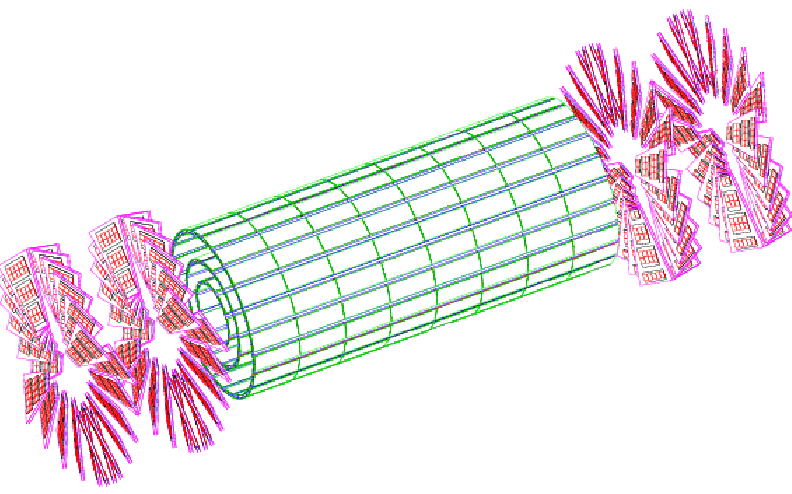
\includegraphics[width=\textwidth]{Images/CMS/PixelDiagram2.png}
    \caption{A diagram of the Phase-1 pixel detector with the BPIX drawn in green and the FPIX drawn in magenta.}
    \label{fig:PixelDiagram}
\end{figure}

\subsubsection{Strip tracker} \label{sec:StripTracker}

Surrounding the pixel detector is the silicon strip tracker \cite{SiliconStrip} which serves the same function as the pixel tracker and covers hits in the same pseudorapidity $|\eta|<2.5$ range. The silicon strip detector is also built with a modular structure, with 15,148 tracker modules each housing one or two silicon sensors totaling 24,244 strip sensors. The silicon strip tracker is divided into four sections: inner barrel (TIB), outer barrel (TOB), inner disks (TID), and outer endcaps (TEC). The TIB and TOB consist of four and six concentric shells respectively, while the TID consists of three disks in each of the forward regions, divided into three concentric rings, and the TEC consists of nine disks with four to seven concentric rings, also in the forward regions. A schematic of the silicon strip detector is provided in Fig.~\ref{fig:StripDiagram} showing the pseudorapidity coverage.

\begin{figure}[H]
    \centering
    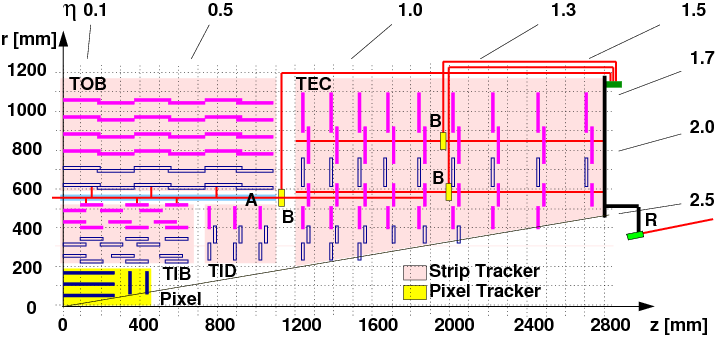
\includegraphics[width=\textwidth]{Images/CMS/TrackerQuadrant.png}
    \caption{A schematic cutaway showing one quadrant of the strip and pixel trackers.}
    \label{fig:StripDiagram}
\end{figure}

\subsection{Calorimeters} \label{sec:Calorimeters}
To measure the energy deposits of electromagnetic particles (e.g., electrons, photons) and hadrons (e.g., neutrons, mesons, jets), CMS relies on two calorimeters: the electromagnetic calorimeter and the hadronic calorimeter, both surrounding the CMS tracker and inside the solenoid magnet.

\subsubsection{The Electromagnetic Calorimeter} \label{sec:ECAL}
% Introduce detector, location, basic info (e.g., chamber count)
Immediately surrounding the CMS tracker is the CMS Electromagnetic Calorimeter (ECAL) \cite{ECALTDR}, which allows CMS to measure the energy deposits left by electrons and photons: highly-favored decay modes of the Higgs boson and critical in its discovery. To optimize performance, the ECAL was designed with the following performance goals: excellent energy and spacial resolution, hermeticity and high-granularity, fast particle identification and fast energy and isolation measurements at trigger-level, a wide energy range (\SI{5}{GeV} to \SI{5}{TeV}), and high radiation tolerance. Energy showers from electrons and photons are measured by an array of lead tungstate (PbWO$_4$) scintillating crystals (Fig.~\ref{fig:ECAL}, left). The ECAL is fully hermetic, composed of a barrel (EB) with a pseudorapidity coverage of $|\eta|<1.48$ and two endcaps (EE) that extend the range to $|\eta|<3.0$, (Cutaways of the EE and EB are shown on the right of Fig.~\ref{fig:ECAL}). Within the EB, crystals are grouped into 36 supermodules each containing 1700 crystals, and in each EE crystals are grouped into two dees with 3662 crystals in each, for a total of 75848 crystals in the ECAL. Crystals are oriented in a projective geometry, with an approximately $3^{\circ}$ tilt to avoid aligning crystal gaps with radial particle trajectories. Lining the inner faces of the EE dees in the range $1.65<|\eta|<2.6$ are preshower detectors (ES) made from lead absorbers and silicon strip sensors. A diagram of the ECAL showing the supermodule placement and pseudorapidity coverage is provided on the right of Fig.~\ref{fig:ECALDiagram}.

\begin{figure}[H]
    \centering
    \resizebox{1\textwidth}{!}{
    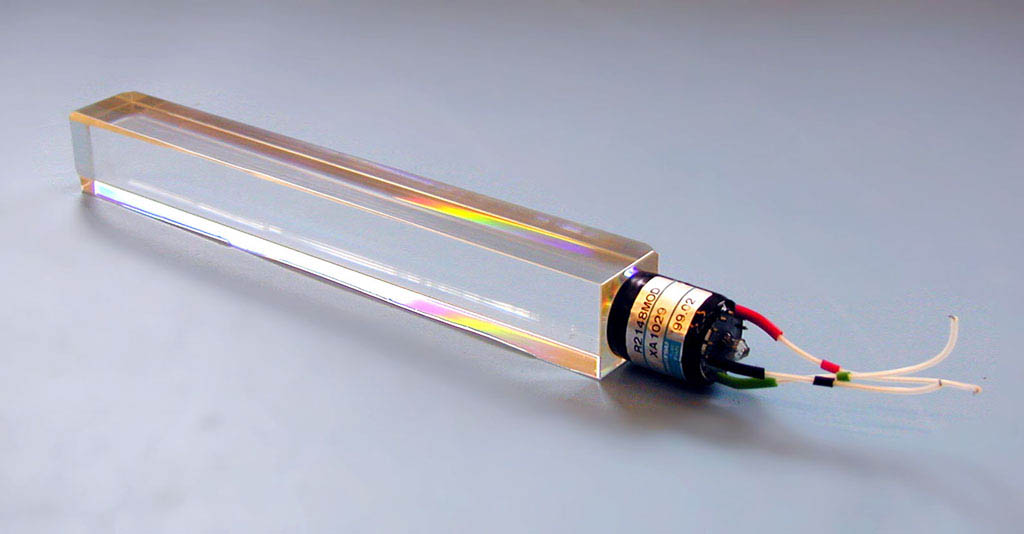
\includegraphics[height=\textwidth]{Images/CMS/ECALCrystal.jpg}
    \quad
    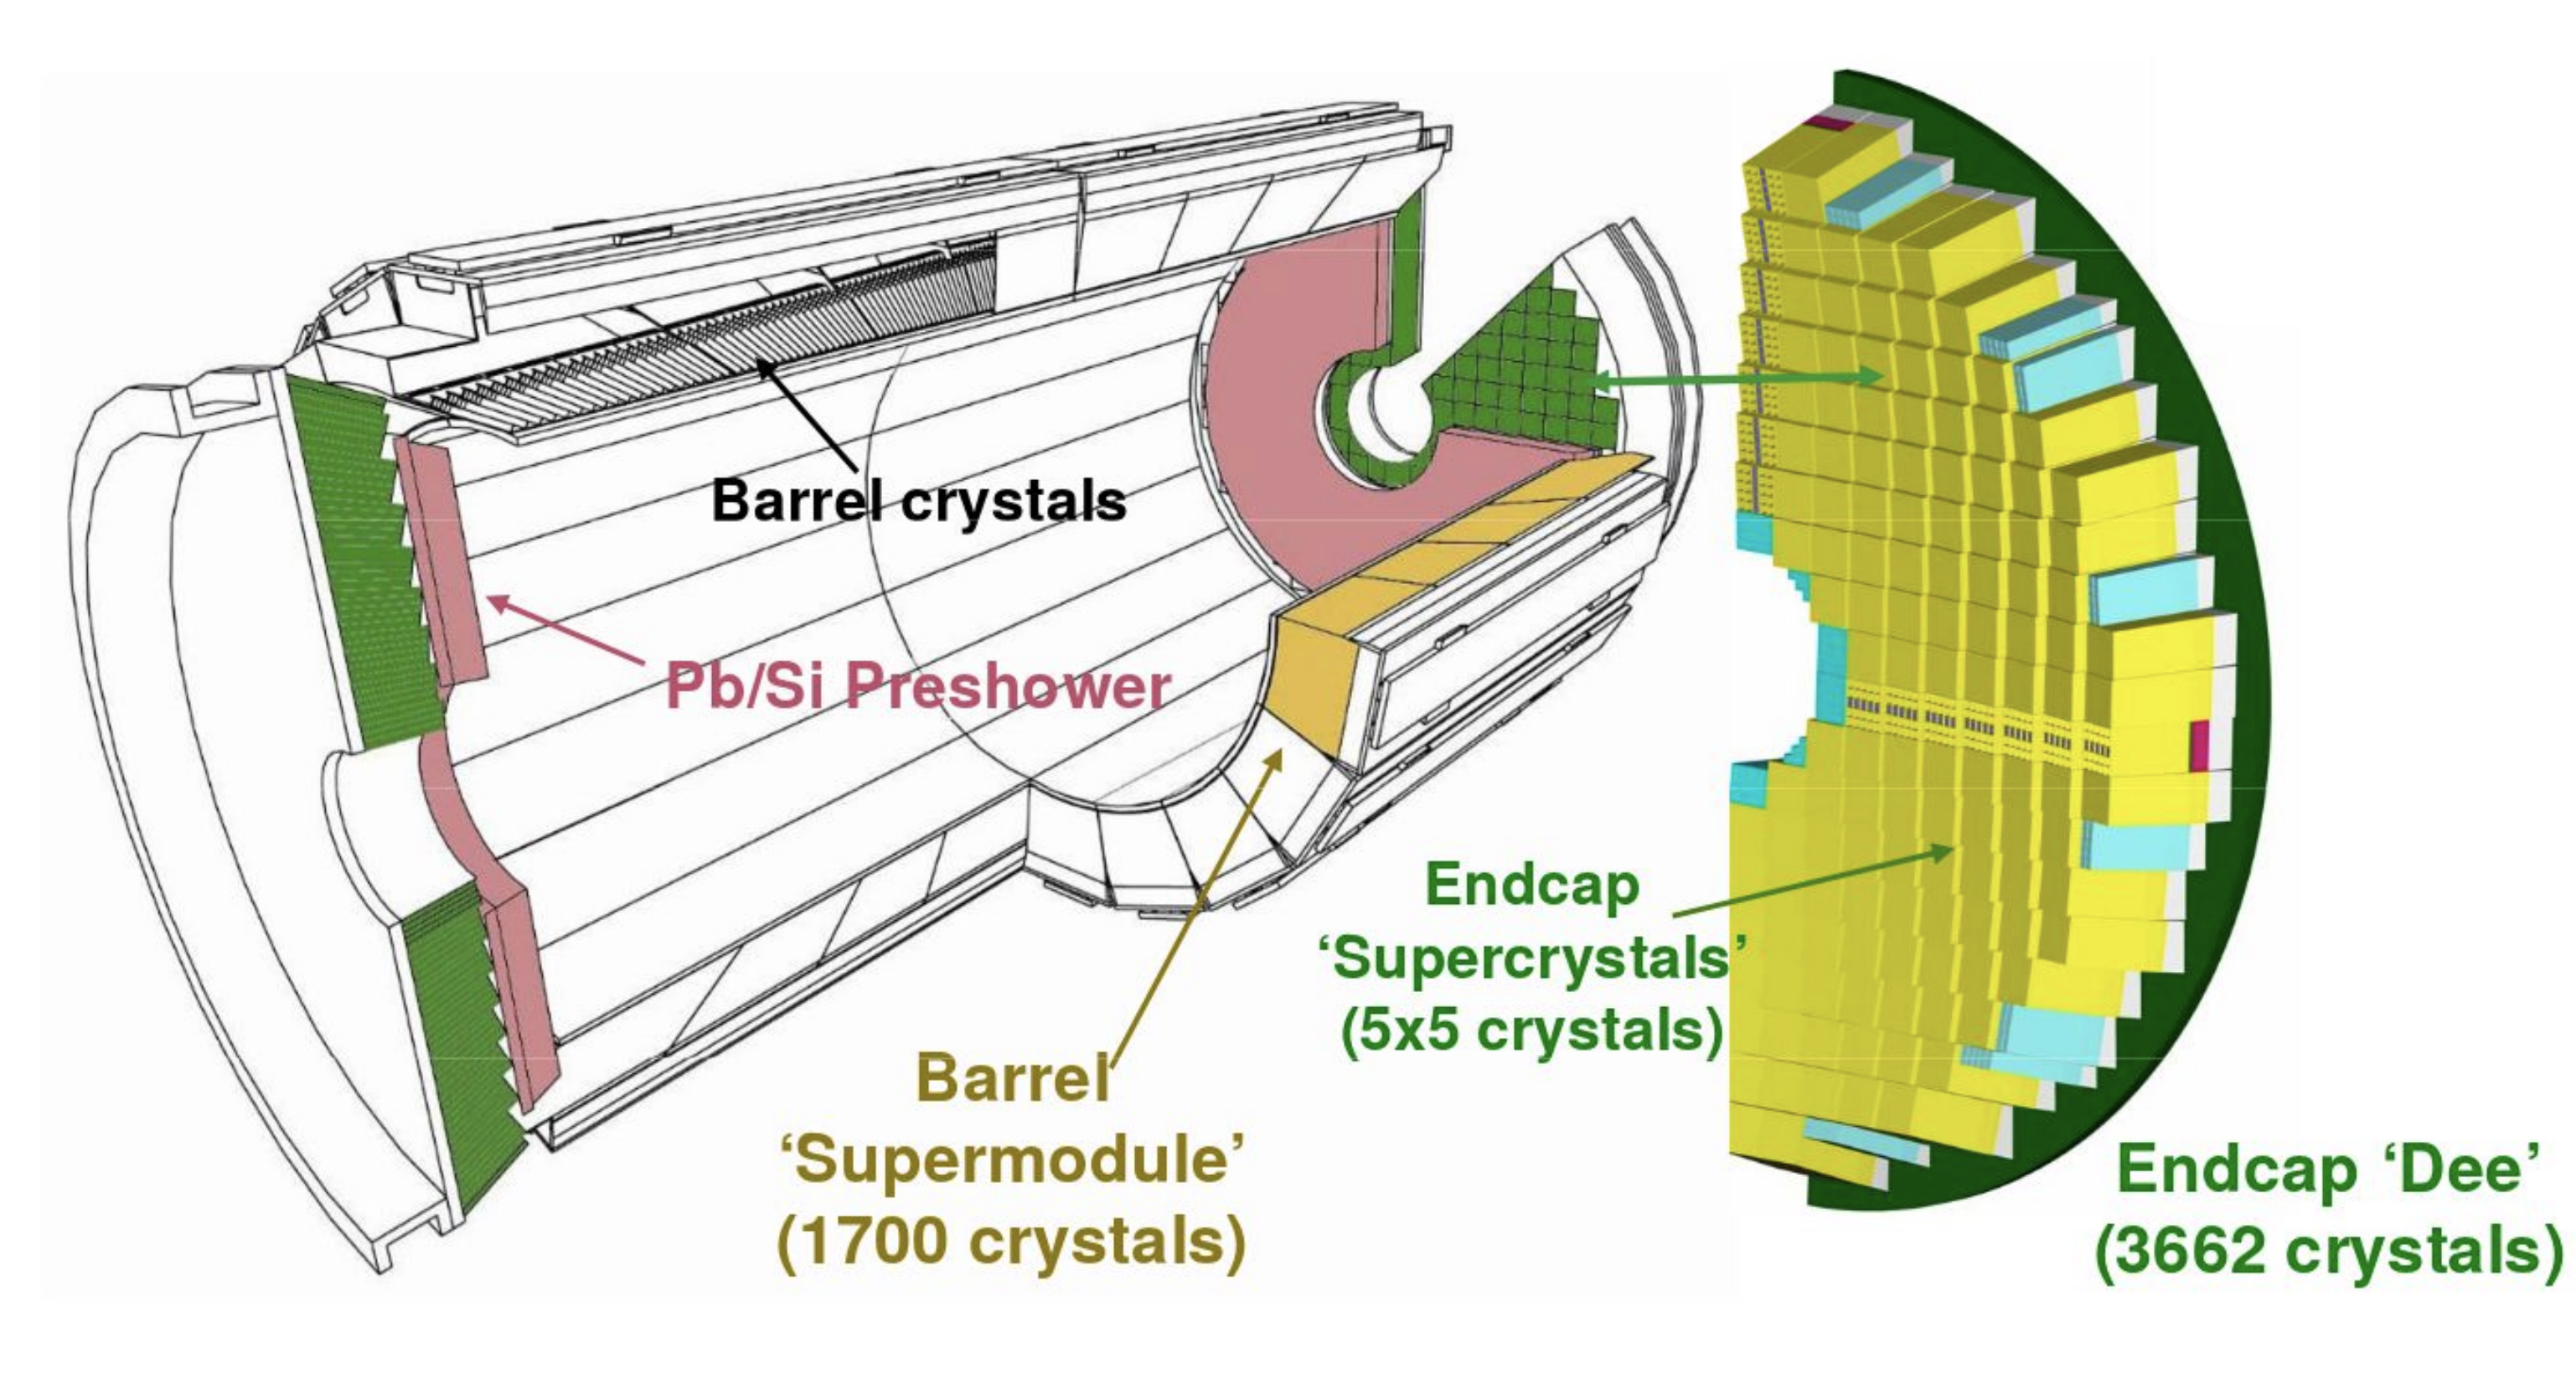
\includegraphics[height=\textwidth]{Images/CMS/ECALDiagram2.png}
    }
    \caption{Left: A photograph of an ECAL crystal. Right: A cutaway showing the orientation of the ECAL supermodules in the barrel and endcap.}
    \label{fig:ECAL}
\end{figure}

\begin{figure}[H]
    \centering
    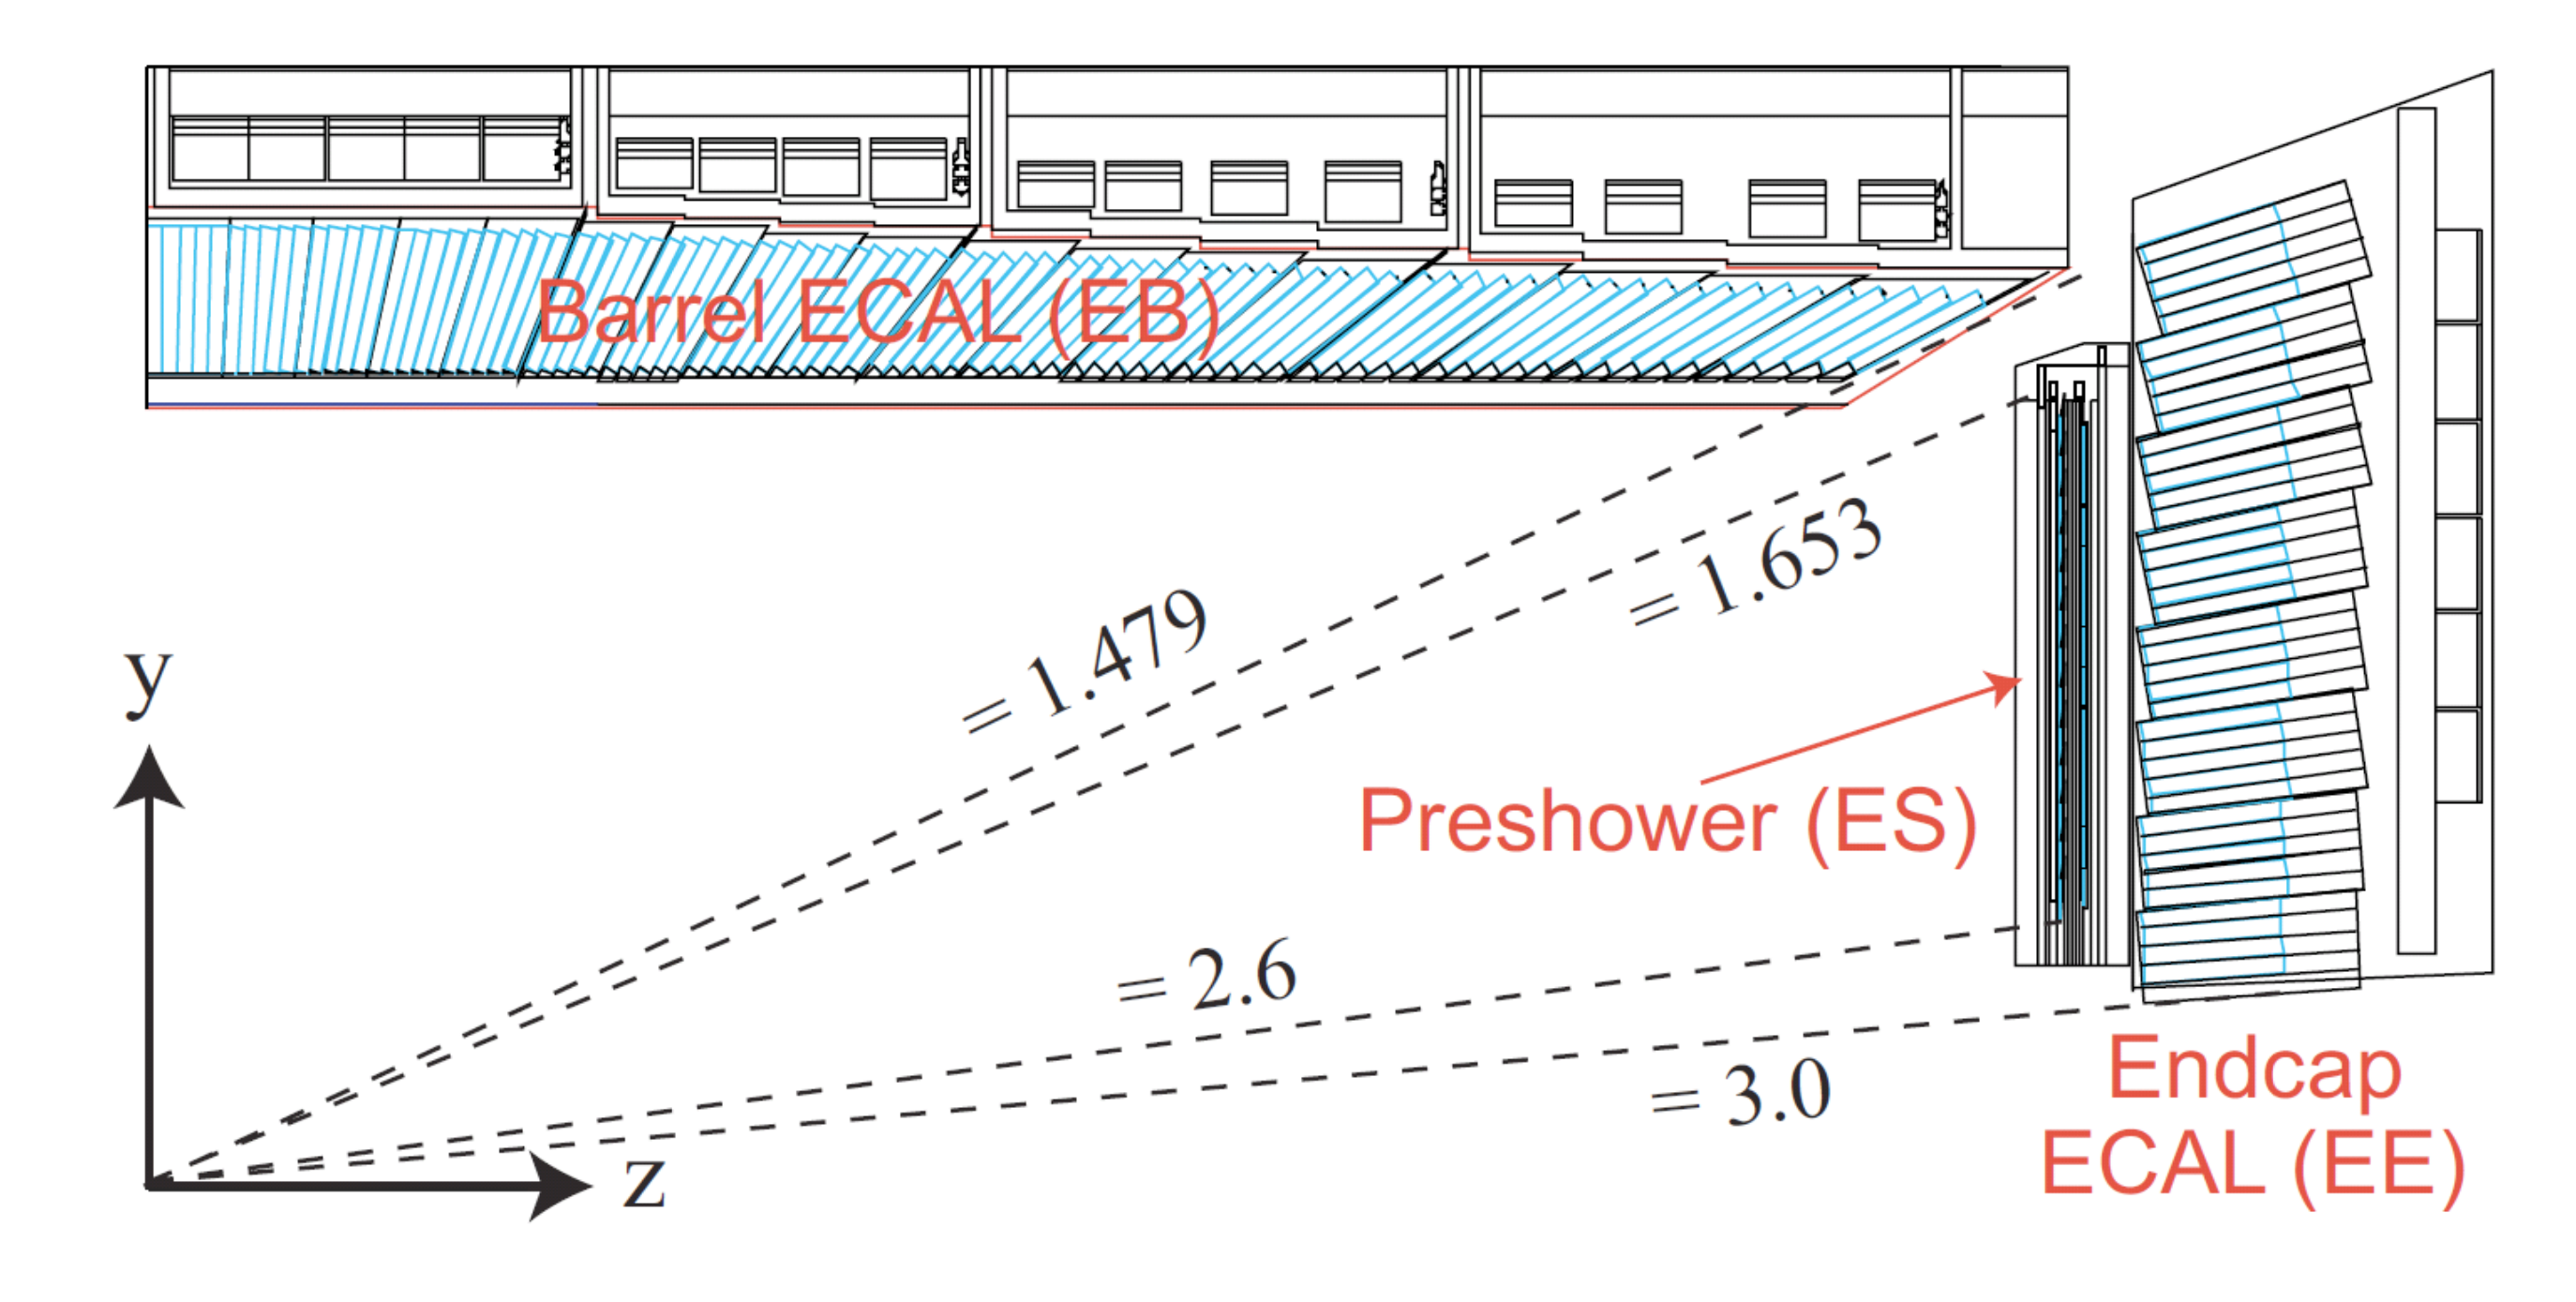
\includegraphics[width=\textwidth]{Images/CMS/ECALDiagram.png}
    \caption{A schematic cutaway showing one quadrant of the ECAL.}
    \label{fig:ECALDiagram}
\end{figure}

\subsubsection{The Hadron Calorimeter} \label{sec:HCAL}
% Introduce detector, location, basic info (e.g., chamber count)
% What is the technology
% Anatomy of a chamber
% How are they arranged in the barrel/endcap
% What do they measure
% Coverage
% Performance

The CMS Hadron Calorimeter (HCAL) \cite{HCALTDR} measures quark, gluon, and neutral particle energy and direction by observing jet energy and missing transverse energy. Within the solenoid magnet, the HCAL is separated into a barrel (HB) and two endcaps (HE), forming the ``central'' HCAL, with a combined pseudorapidity coverage of $|\eta| < 3.0$. An additional two detectors are located outside the solenoid magnet: an array of scintilators that catch the tails of hadronic showers and aid in muon identification called the HCAL Outer calorimeter (HO); and the forward calorimeter (HF), located \SI{6}{m} down the beamline from the ``central'' HCAL (one at each end) and covering the pseudorapidity range $3.0<|\eta|<5.0$, required for accurate missing transverse energy measurements (a diagram showing the arrangement and pseudorapidity coverage of the HCAL and HF is shown in Fig.~\ref{fig:HCALDiagram}). The HB is divided into two half-barrels, each housing 18 wedges ($20^{\circ}$ in $\phi$) of brass alloy absorber plates with a wavelength shifting fiber (WSF) readout. Both the HEs and HFs are composed of quartz fibers embedded in a copper absorber matrix. Optical signals are transmitted to hybrid photo diodes (HPD) in the HB and HE, and by photomultiplier tubes (PMT) in the HFs. A photograph of the HB during installation is shown in Fig.~\ref{fig:HCAL}.

\begin{figure}[H]
    \centering
    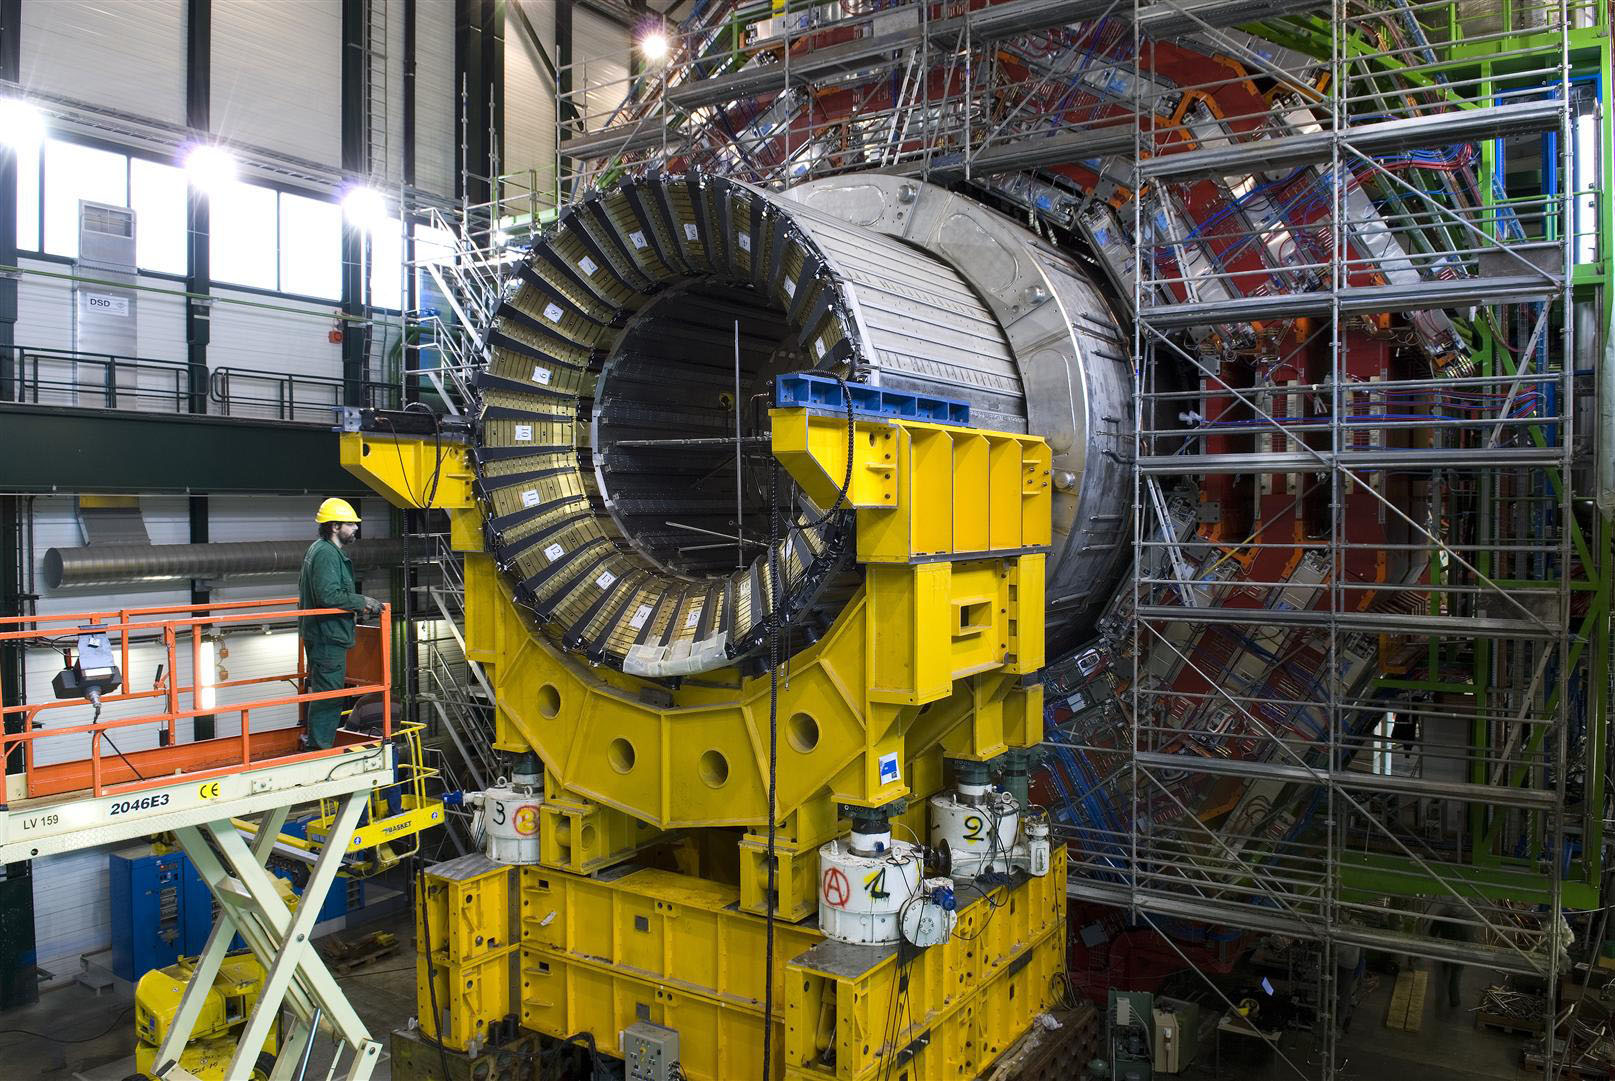
\includegraphics[width=\textwidth]{Images/CMS/HCal.jpg}
    \caption{A photograph showing the HCAL barrel during installation.}
    \label{fig:HCAL}
\end{figure}

\begin{figure}[H]
    \centering
    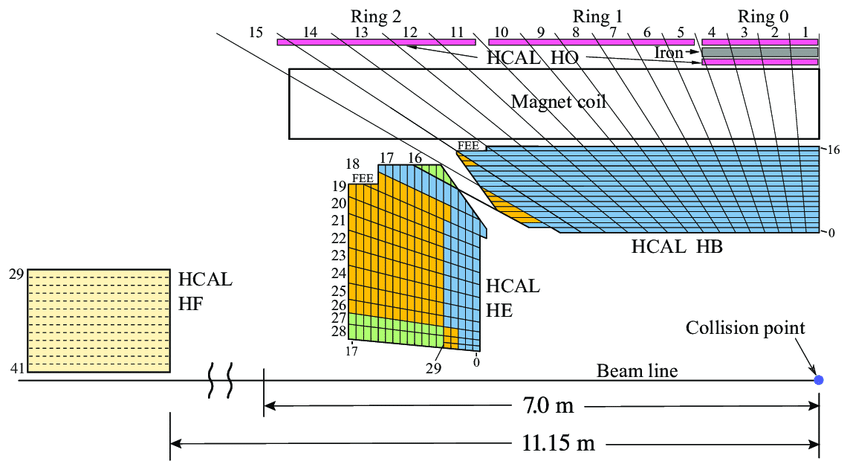
\includegraphics[width=\textwidth]{Images/CMS/HCALDiagram.png}
    \caption{A schematic cutaway showing one quadrant of the HCAL.}
    \label{fig:HCALDiagram}
\end{figure}

\subsection{Solenoid magnet} \label{sec:SolenoidMagnet}


Enclosing the CMS tracker and calorimeters is a \SI{3.8}{T} superconducting solenoid magnet---the most powerful in the world. The cylindrical structure of the solenoid measures \SI{6}{m} in internal diameter and \SI{12.5}{m} long, seen in the photograph in Fig.~\ref{fig:Magnet}. The high magnetic field inside the solenoid is necessary to induce sufficient bending of charged particle trajectories in the transverse plane so precise $p_T$ measurements can be made by the tracker. Outside the solenoid is a ferromagnetic return yoke made of construction steel, divided into five wheels in the barrel region labeled YBw and three disks n in each (positive and negative) endcap labeled YE$\pm$n. The return yoke induces a strong magnetic field within the muon system (mounted to the return yoke) that improves the $p_T$ measurements of muons. The direction of the bending of particles inside the tracker and muon systems is also used to identify the charge sign. The solenoid magnet also serves as a support structure for the \SI{10000}{ton} steel return yoke.

\begin{figure}[H]
    \centering
    {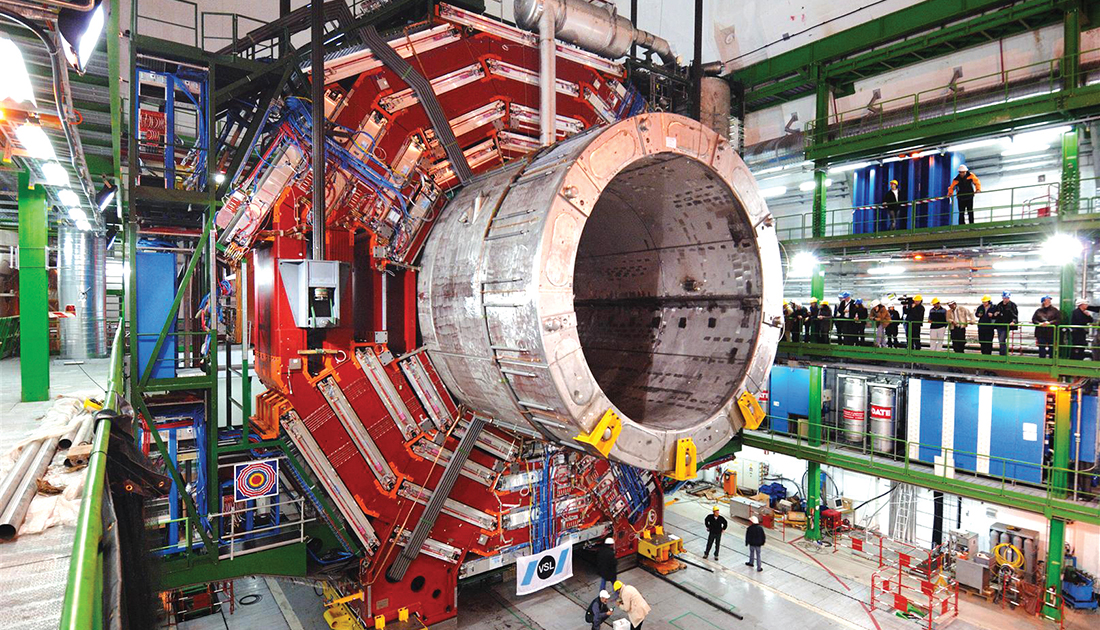
\includegraphics[width=\textwidth]{Images/CMS/Magnet.jpg}}
    \caption{The solenoid magnet of CMS together with a wheel of the steel return yoke.}
    \label{fig:Magnet}
\end{figure}


\subsection{Muon system} \label{sec:MuonSystem}
The muon system \cite{MuonTDR} is responsible for recording the momenta of muons in the outer-most layer of CMS. As muons provide a clean signature in many physics analyses, obtaining high-resolution measurements of muon momenta is critical. It comprises four separate technologies that provide redundancy in both the barrel and endcap regions. The subsystems are the Drift Tubes (DTs) in the barrel, the Cathode Strip Chambers (CSCs) in the endcap regions, the Resistive Plate Chambers (RPCs) in both the barrel and endcaps, and as of Run 3, the Gas Electon Multipliers (GEMs) located in the outer-most layer of the endcaps. Each subsytem uses a different technology and records muon hits separately, with reconstruction combining the information from all the subsystems. The muon barrel (MB) system is divided into four concentric shells, or stations, in each of the five wheels of the CMS barrel, labeled from inner-most to outer-most (along the $r$-coordinate): MB1, MB2, MB3, and MB4. Similarly, the muon endcap (ME) system is arranged into four disks in both the plus and minus endcaps, also called stations, labeled from inner-most to outer-most (along the $z$-coordinate): ME$\pm$1, ME$\pm$2, ME$\pm$3, and ME$\pm$4 ($\pm$ of course identifies the plus or minus endcap). Figure~\ref{fig:MuonSystem} shows a diagram including each subsytem and the pseudorapidity coverage of the muon system.

\begin{figure}[H]
    \centering
    {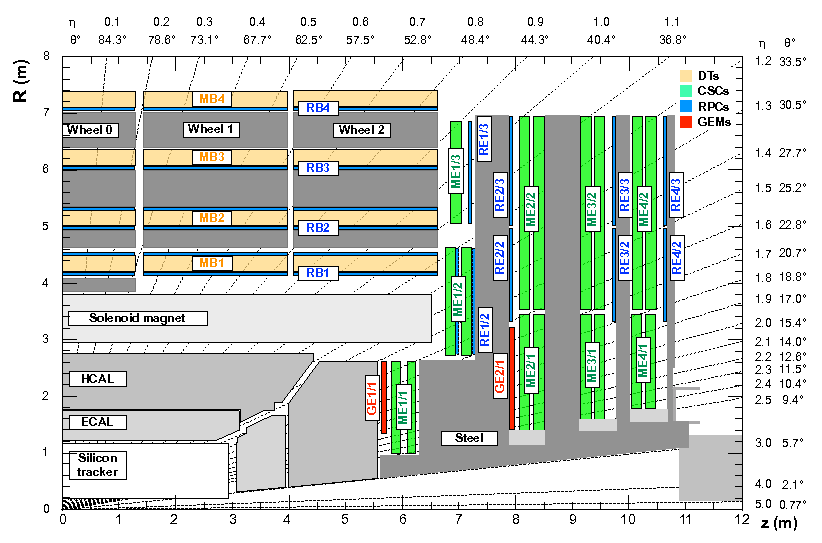
\includegraphics[width=1\textwidth]{Images/CMS/MuonSystem.png}}
    \caption{A cutaway schematic of one quadrant of the muon system. Included are the CSCs, DT chambers, RPCs, and GEM detectors.}
    \label{fig:MuonSystem}
\end{figure}

\subsubsection{Cathode Strip Chambers} \label{sec:CSC}
% Introduce detector, location, basic info (e.g., chamber count)
% What is the technology
% Anatomy of a chamber
% How are they arranged in the barrel/endcap
% What do they measure
% Coverage
% Performance

Providing coverage in the plus and minus MEs within $0.9<|\eta|<2.4$ are the Cathode Strip Chambers (CSCs), which occupy the four ME stations along with RPCs. CSCs are labeled by ME station $\pm$n, then by ring m, like ``ME$\pm$n/m.'' In ME$\pm$2 to ME$\pm$4, each station consists of two concentric rings of CSCs, while ME$\pm$1 supports three rings of chambers (see Fig.~\ref{fig:CSC}). All rings contain 36 chambers, except for the outer-most rings of stations 2-4 (ME$\pm$2/2, ME$\pm$3/2, and ME$\pm$4/2) which hold only 18 chambers, for a total of 540 CSCs. Within each ring, CSCs are azimuthally overlapping with no gaps, offering full $\phi$ coverage. Each chamber is constructed from seven layers of polycarbonate honeycomb panels, with a gas mixture of 50\% Ar, 40\% CO2, and 10\% CF4 filling the six gaps between the panels. Embedded in a thin FR4 (fire-resistant fiberglass epoxy) surface on each panel are radially-extended cathode strips. Within each gap are azimuthally-running anode wires supplied with \SIrange{2.9}{3.5}{kV} of voltage. Muons passing through a chamber will locally ionize the gas in each gap, while the high voltage will induce a charge avalanche that drifts toward the cathode strips and an image charge will drift toward the anode wires (see Fig.~\ref{fig:CSCDiagram}). Each chamber provides a spacial resolution of \SIrange{50}{140}{\micro\meter} (depending on the chamber) and a timing resolution of \SI{3}{ns}.

\begin{figure}[H]
    \centering
    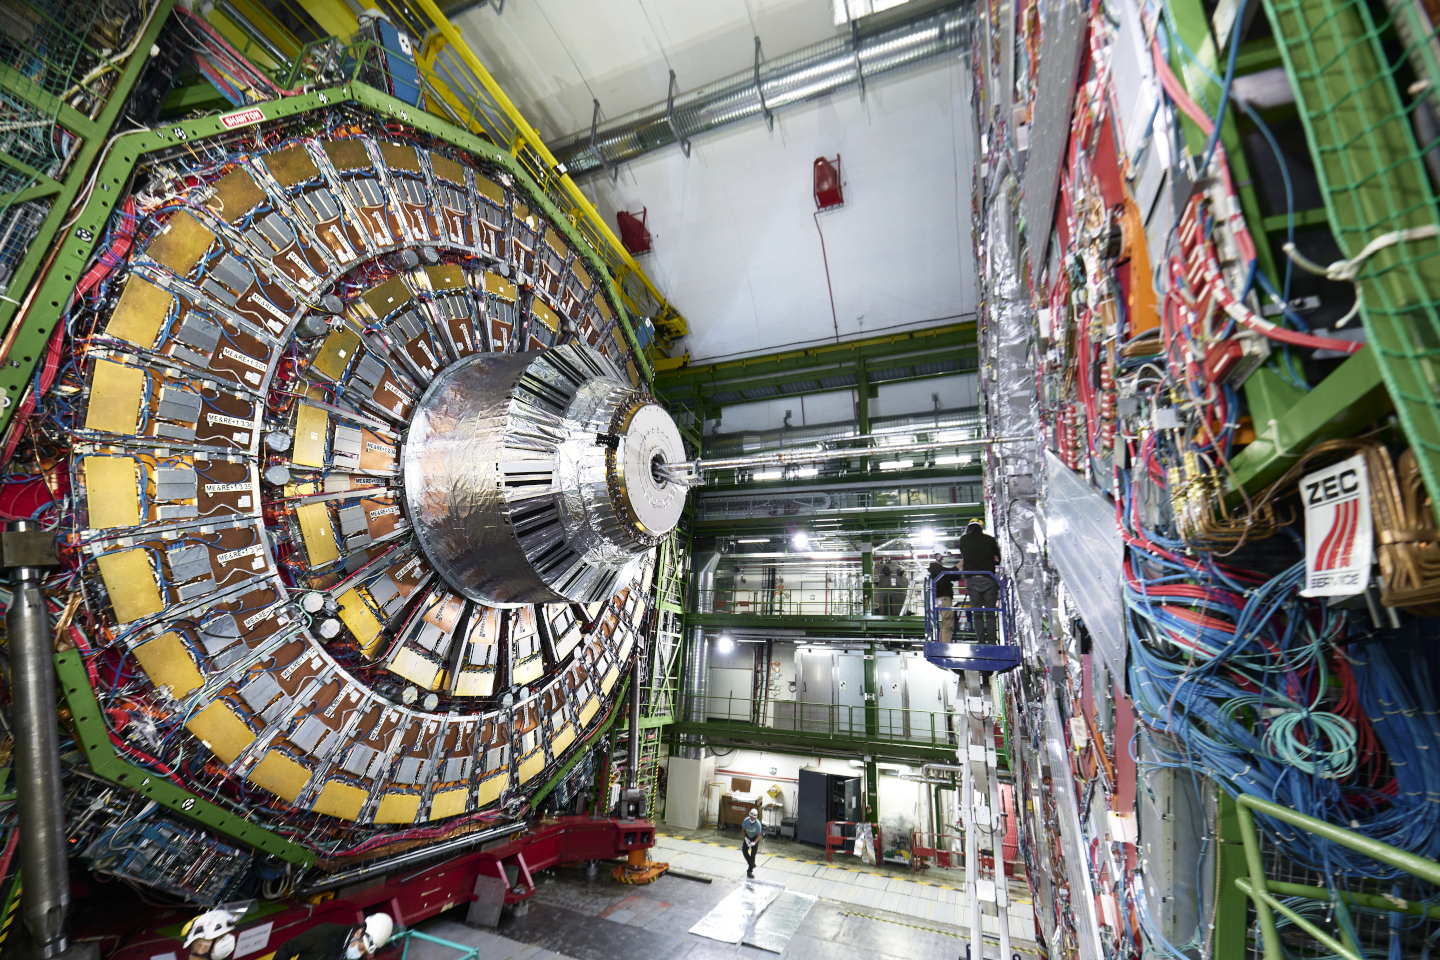
\includegraphics[width=1\textwidth]{Images/CMS/CSC.jpg}
    \caption{A photograph of CSCs mounted to the first endcap station.}
    \label{fig:CSC}
\end{figure}

\begin{figure}[H]
    \centering
    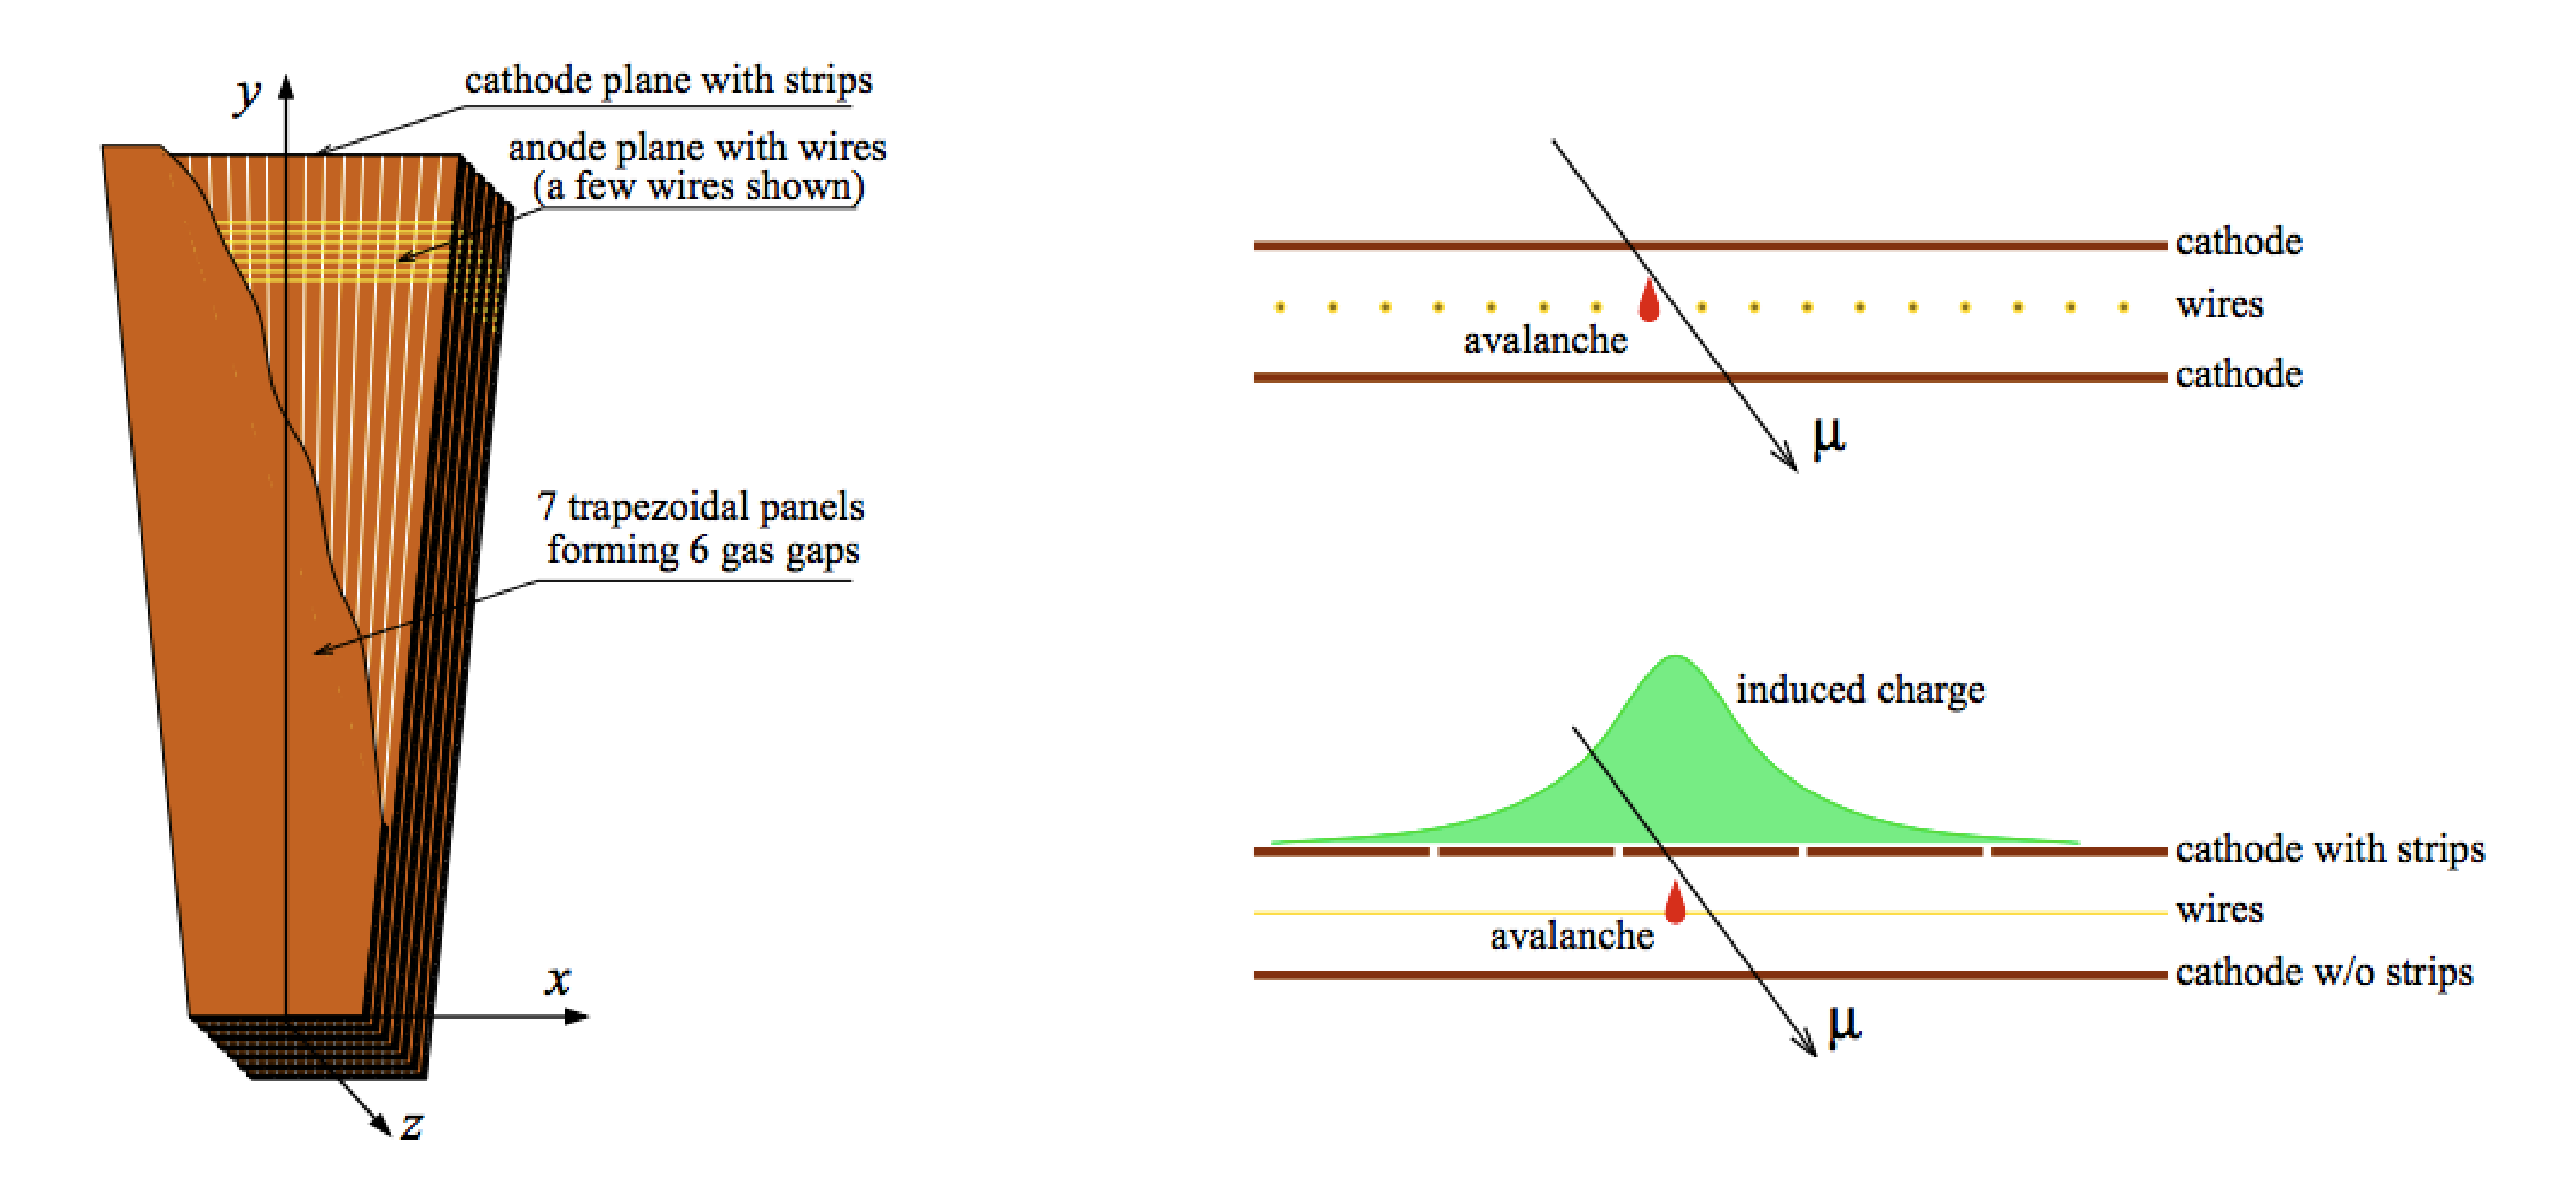
\includegraphics[width=\textwidth]{Images/CMS/CSCDiagram.png}
    \caption{Left: A schematic of a CSC. Right: A muon passing through a CSC will induce a charge avalanche.}
    \label{fig:CSCDiagram}
\end{figure}

\subsubsection{Drift Tubes} \label{sec:DT}

% Introduce detector, location, basic info (e.g., chamber count)
% What is the technology
% Anatomy of a chamber
% How are they arranged in the barrel/endcap
% Coverage
% What do they measure
% Precision
% Performance

Located in the MB are 250 Drift Tube (DT) chambers, layered between RPCs, and arranged to provide coverage within $|\eta|<1.2$ overlapping with the CSC coverage in the muon endcaps (see Fig.~\ref{fig:DT}). DT chambers are labeled by MB station n, then by wheel w, like ``MBn$\pm$w.'' A single DT consists of a long aluminum drift cell filled with a gas mixture of 85~\% Ar and 15~\% CO2 and a central anode wire strung length-wise inside the cell held at \SI{+3600}{V}. Electrode strips held at \SI{+1800}{V} and cathode strips held at \SI{-1200}{V} line the walls of each cell and help shape the electric field inside (see the diagram in Fig.~\ref{fig:DTDiagram}). In MB1-MB3, the DT chambers are grouped into three collections of four consecutive, stagered layers of drift tubes called Super Layers (SLs), while in MB4 there are only two SLs per chamber. The inner-most and outer-most SL in a DT chamber measure $r$-$\phi$ coordinates in the bending plane, while the middle SL measures along the $z$-coordinate. Between the outer-most and middle SL is a honeycomb layer that produces a $\SI{28}{cm}$ separation of measurements in the bending plane, which aid in determining muon track bending. In MB4, DT chambers consist only of the two SLs measuring the $r$-$\phi$-coordinate, with no honeycomb spacer or $z$-coordinate SL. The spatial resolution per cell is at least \SI{250}{\micro\meter}, corresponding to a roughly \SI{100}{\micro\meter} resolution per chamber, while the time resolution per DT chamber is \SI{2}{ns}.

\begin{figure}[H]
    \centering
    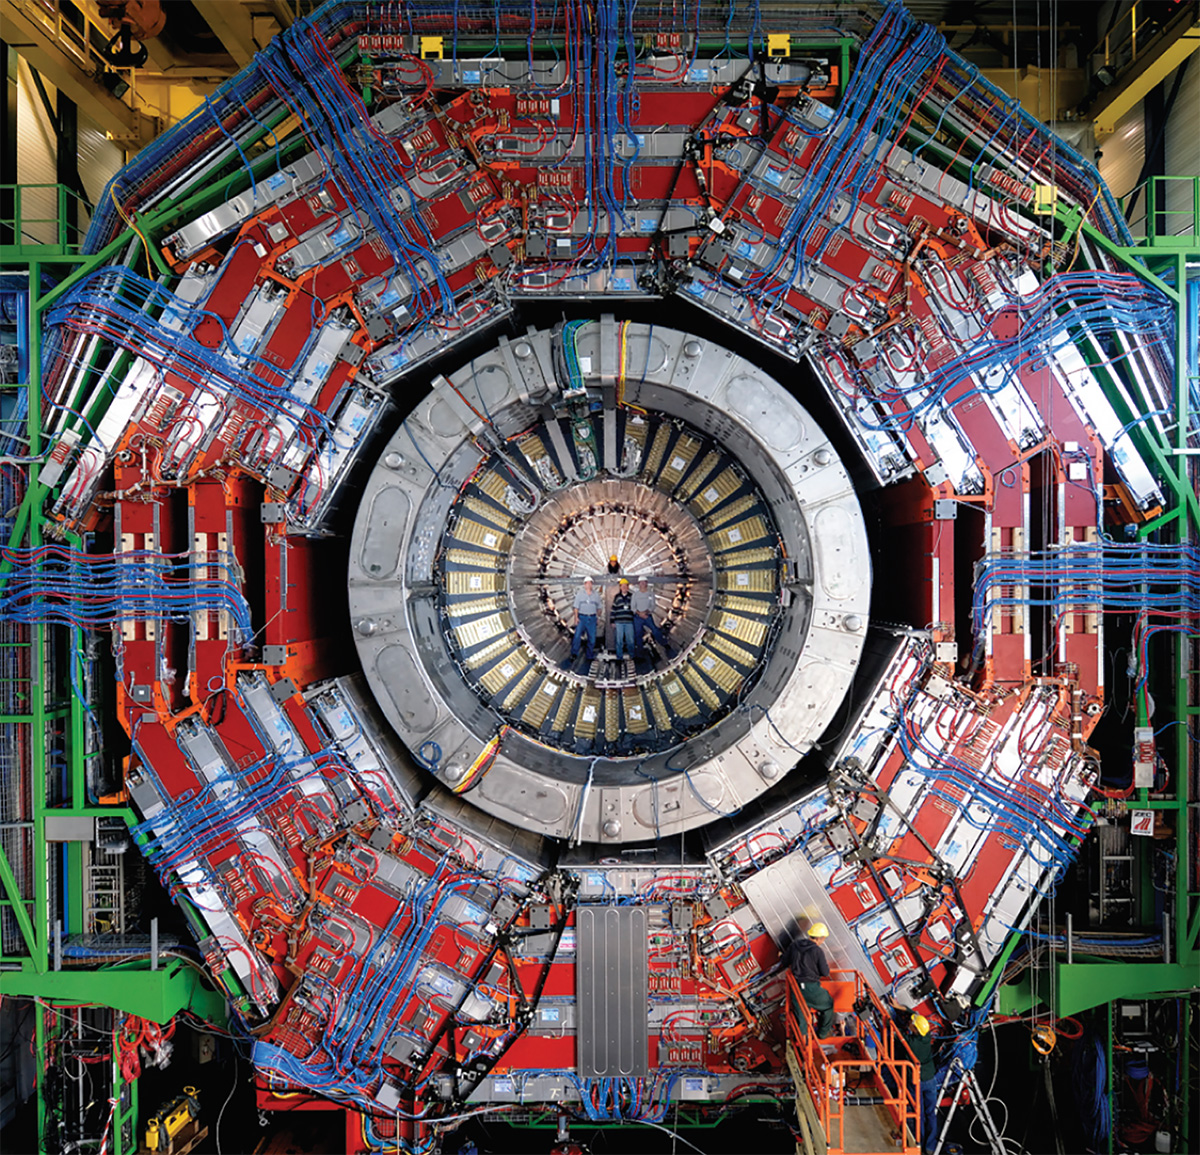
\includegraphics[width=\textwidth]{Images/CMS/DT.jpg}
    \caption{A photograph of DT chambers (silver boxes) installed in the return yoke (red structure) of a wheel in the muon barrel.}
    \label{fig:DT}
\end{figure}

\begin{figure}[H]
    \centering
    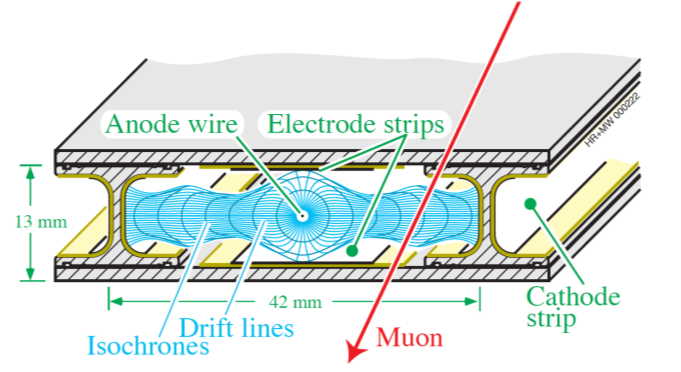
\includegraphics[width=1\textwidth]{Images/CMS/DTDiagram.png}
    \caption{A diagram of a single DT chamber.}
    \label{fig:DTDiagram}
\end{figure}

\subsubsection{Resistive Plate Chambers} \label{sec:RPC}
% Introduce detector, location, basic info (e.g., chamber count)
% What is the technology
% Anatomy of a chamber
% How are they arranged in the barrel/endcap
% What do they measure
% Coverage
% Performance

Complementing the DT chambers and CSCs are the Resistive Plate Chambers (RPCs) located in both the MB and ME (shown in Fig.~\ref{fig:RPC}). RPCs have two naming conventions, depending on the region of the detector they occupy: in the barrel, ``RBn$\pm$w,'' and in the endcaps, ``RE$\pm$n/m,'' where ($\pm$)n denotes the MB or ME$\pm$ station (1-4), $\pm$w the MB wheel (1-5), and m the ME ring (1, 2, or 3 in RB$\pm$1; 1or 2 in all other stations). Pseudorapidity coverage by the RPCs overlaps with the other muon subsytems at $0.0 < |\eta| < 1.9$. In stations RB1 and RB2, two RPCs sandwich each DT chamber, while in RB3 and RB4, anywhere from one to four RPCs (depending on the station and sector) are layered on the inside of a single DT chamber. This leads to 480 total RPCs in the barrel. In the endcaps, RPCs are mounted to the opposite side of a yoke disk as the CSCs, forming alternating layers of CSCs and RPCs, and totalling 576 RPCs in the endcaps. Each RPC is a \SI{2}{mm} double-gap chamber, using Bakalite (a high pressure laminate) electrodes, operated in avalanche mode (see the diagram in Fig.~\ref{fig:RPCDiagram}). Electrode strips are longitudinally-running and segmented into two or three parts, depending on the station/sector. A RPC detector is optimized to record accurate timing and fast triggering, as well as identification the associated bunch crossing for a given muon track. Compared to the DTs and CSCs, RPCs have a coarse-grain spatial resolution of only 0.8 to \SI{1.3}{\cm}, but provide excellent timing resolution at \SI{1.5}{\ns}.

\begin{figure}[H]
    \centering
    {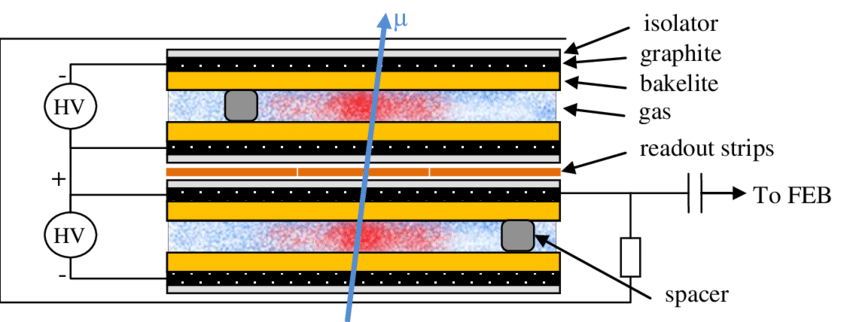
\includegraphics[width=\textwidth]{Images/CMS/RPCDiagram.png}}
    \caption{A diagram of an RPC.}
    \label{fig:RPCDiagram}
\end{figure}


\begin{figure}[H]
    \centering
    {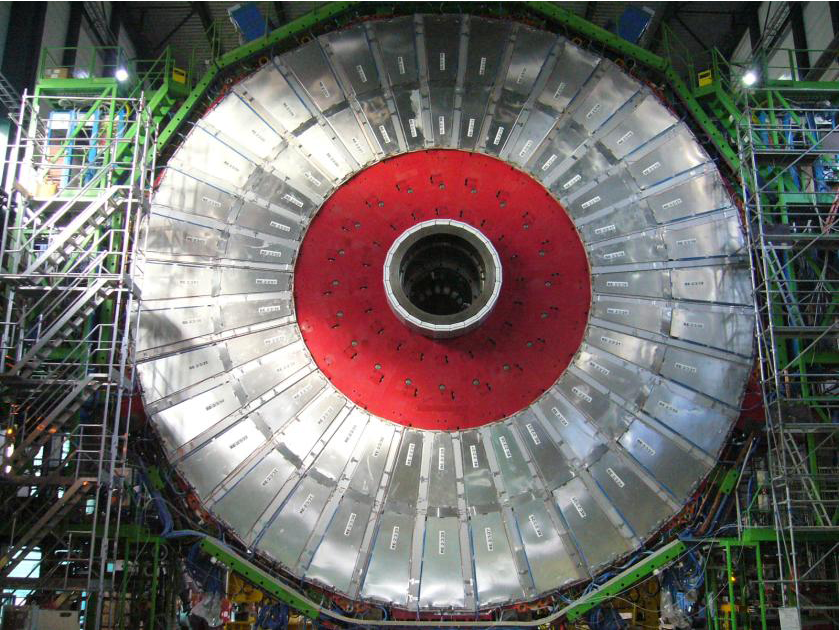
\includegraphics[width=1\textwidth]{Images/CMS/RE.png}}
    \caption{A photograph of RPCs mounted to the second endcap station.}
    \label{fig:RPC}
\end{figure}

\subsubsection{Gas Electron Multipliers} \label{sec:GEM}
During LS2, Gas Electron Multipliers (GEMs) \cite{GEM} were installed as part of the Phase 2 upgrades to the muon system. Located in the very forward regions of each ME and complimenting the CSCs, the GEMs cover the pseudorapidity range of $1.5<|\eta|<2.8$ and are labeled ME$\pm$0, GE$\pm$1/1 and GE$\pm$2/1. Each GEM detector consists of a tripple-layer of copper-cladded polyimide foil into which are etched \SI{70}{\micro \meter} holes spaced \SI{70}{\micro\meter} apart, in a hexagonal geometry, as can be seen in the diagrams in Figs.~\ref{fig:GEMDiagram} and~\ref{fig:GEMDiagram2} (left). A 70 \% Ar and 30 \% CO$_2$ gas mixture fills mm-sized gaps between the foil layers and a voltage is applied is steps ranging from \SI{-3200}{V} to ground (see Fig.~\ref{fig:GEMDiagram2}, right). The foil layers are sandwitched between a drift PCB and a readout PCB with 3072 radial strips. A total of 144 GEM chambers were installed during LS2 occupying the GE$\pm$1/1 station/ring, with the remaining chambers, ME$\pm$0 and GE$\pm$2/1 to be installed in LS3. 

\begin{figure}[H]
    \centering
    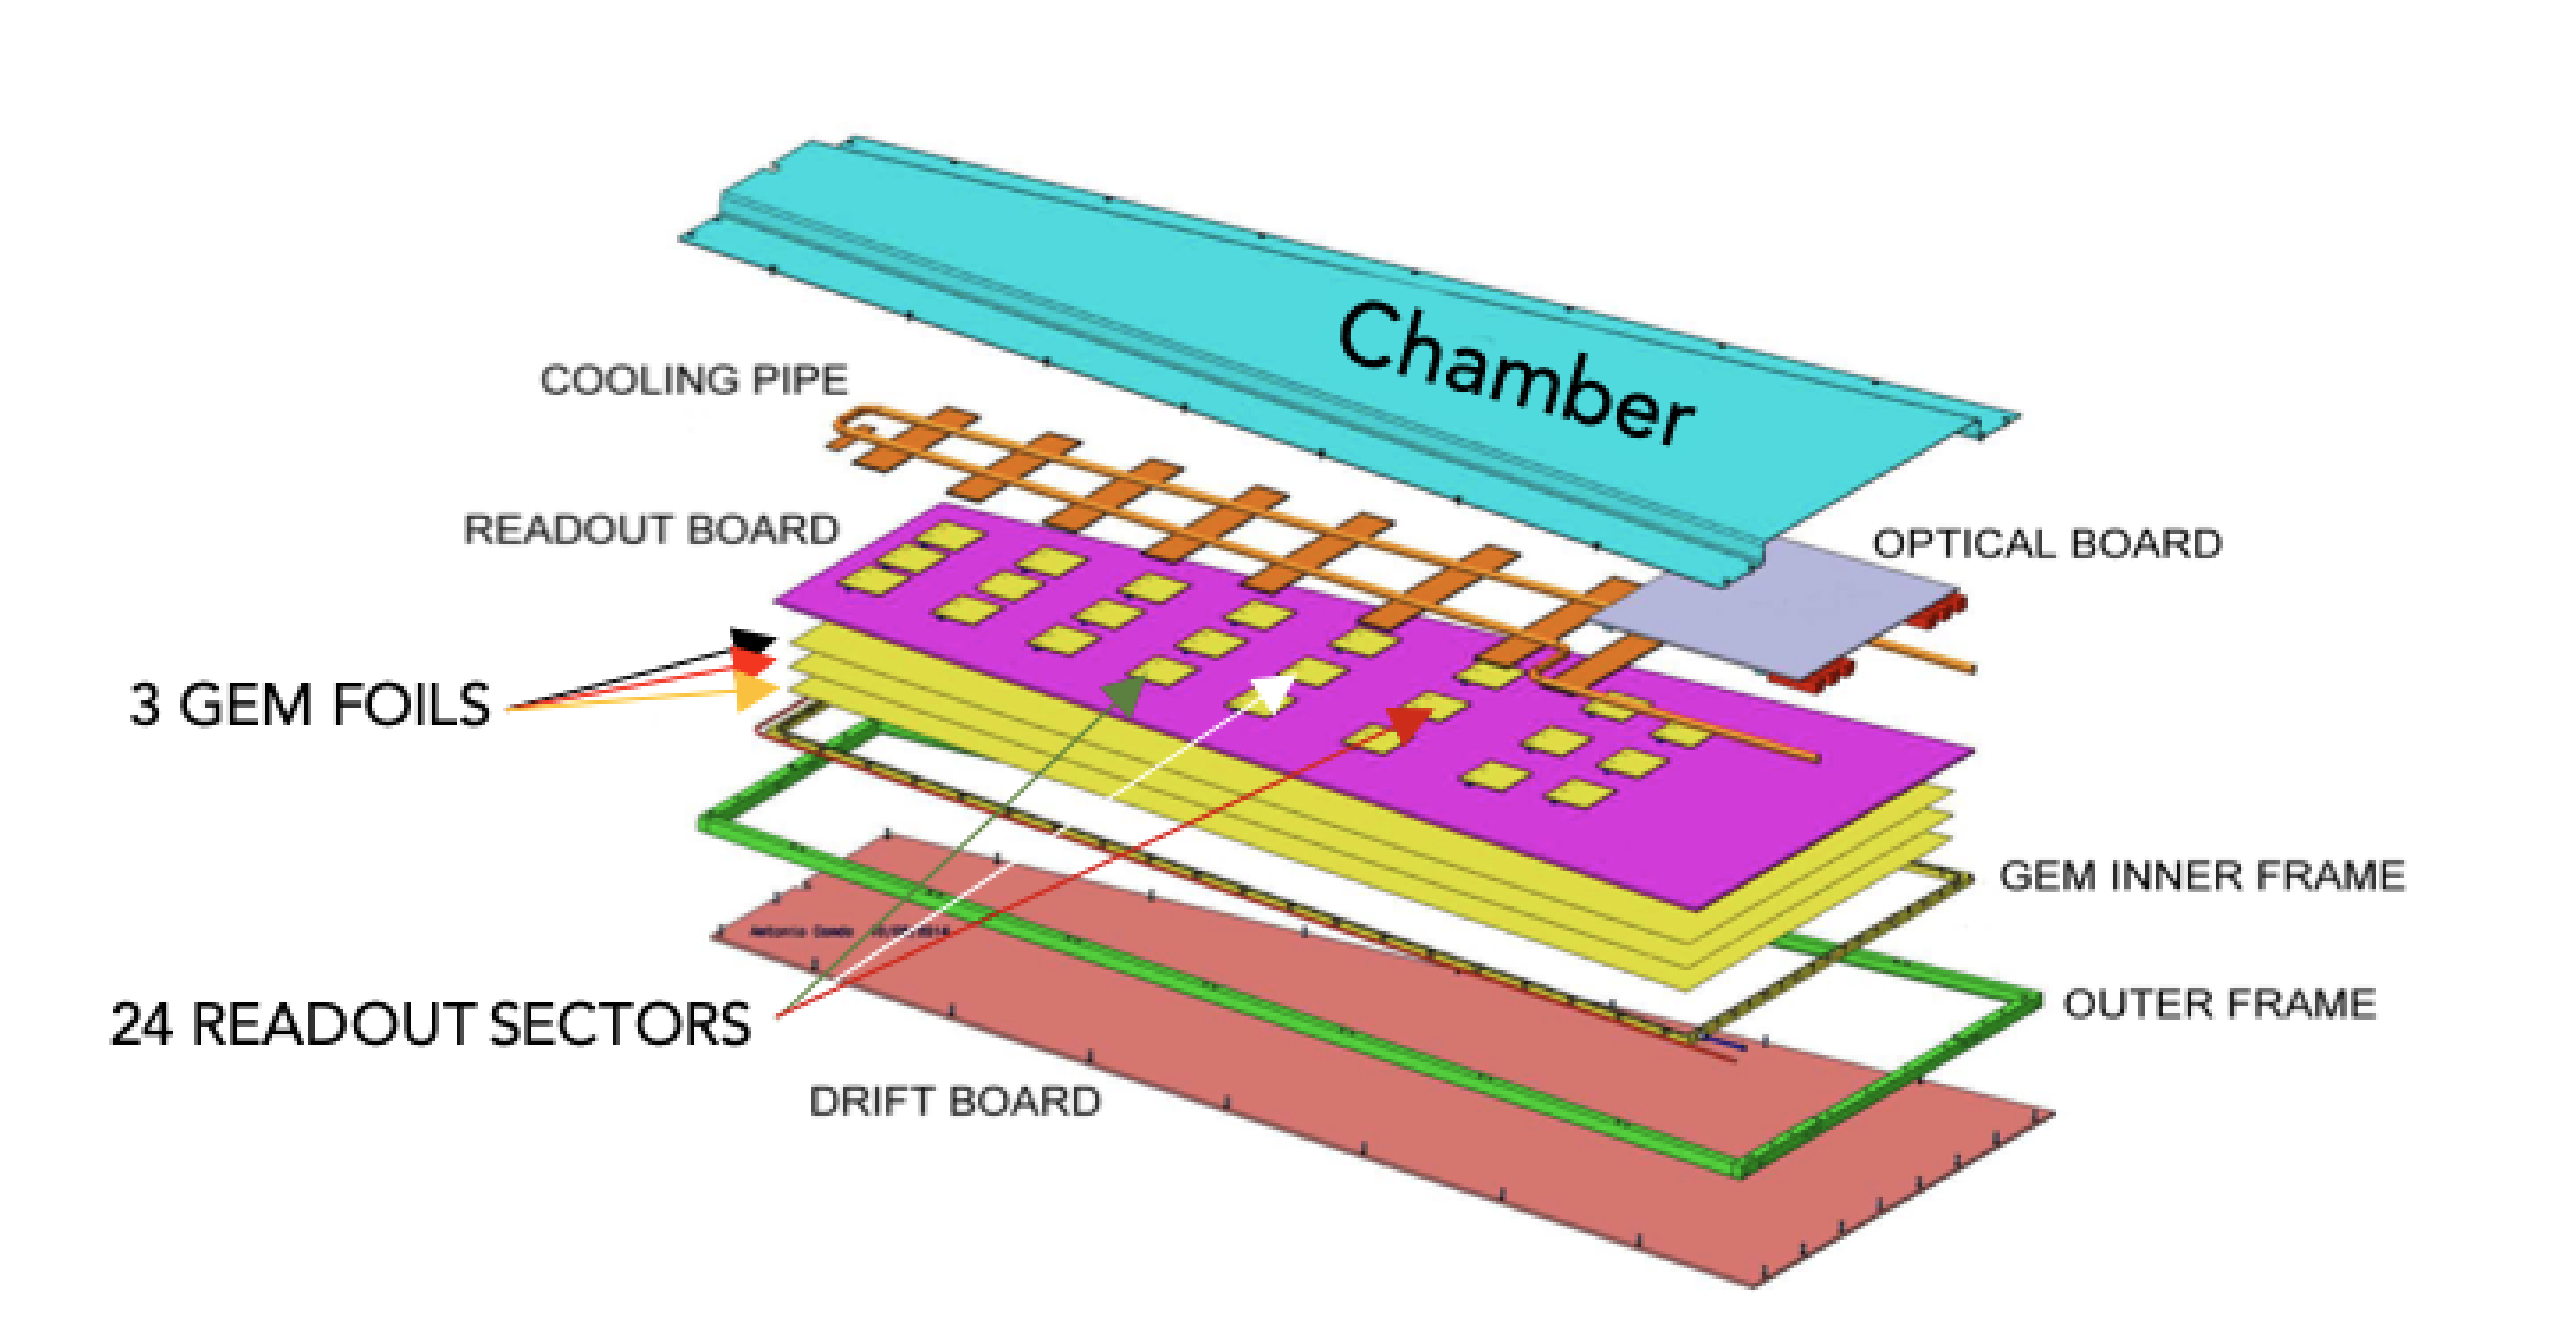
\includegraphics[width=\textwidth]{Images/CMS/GEMDiagram.png}
    \caption{An exploded view of a GEM chamber.}
    \label{fig:GEMDiagram}
\end{figure}

\begin{figure}[H]
    \centering
    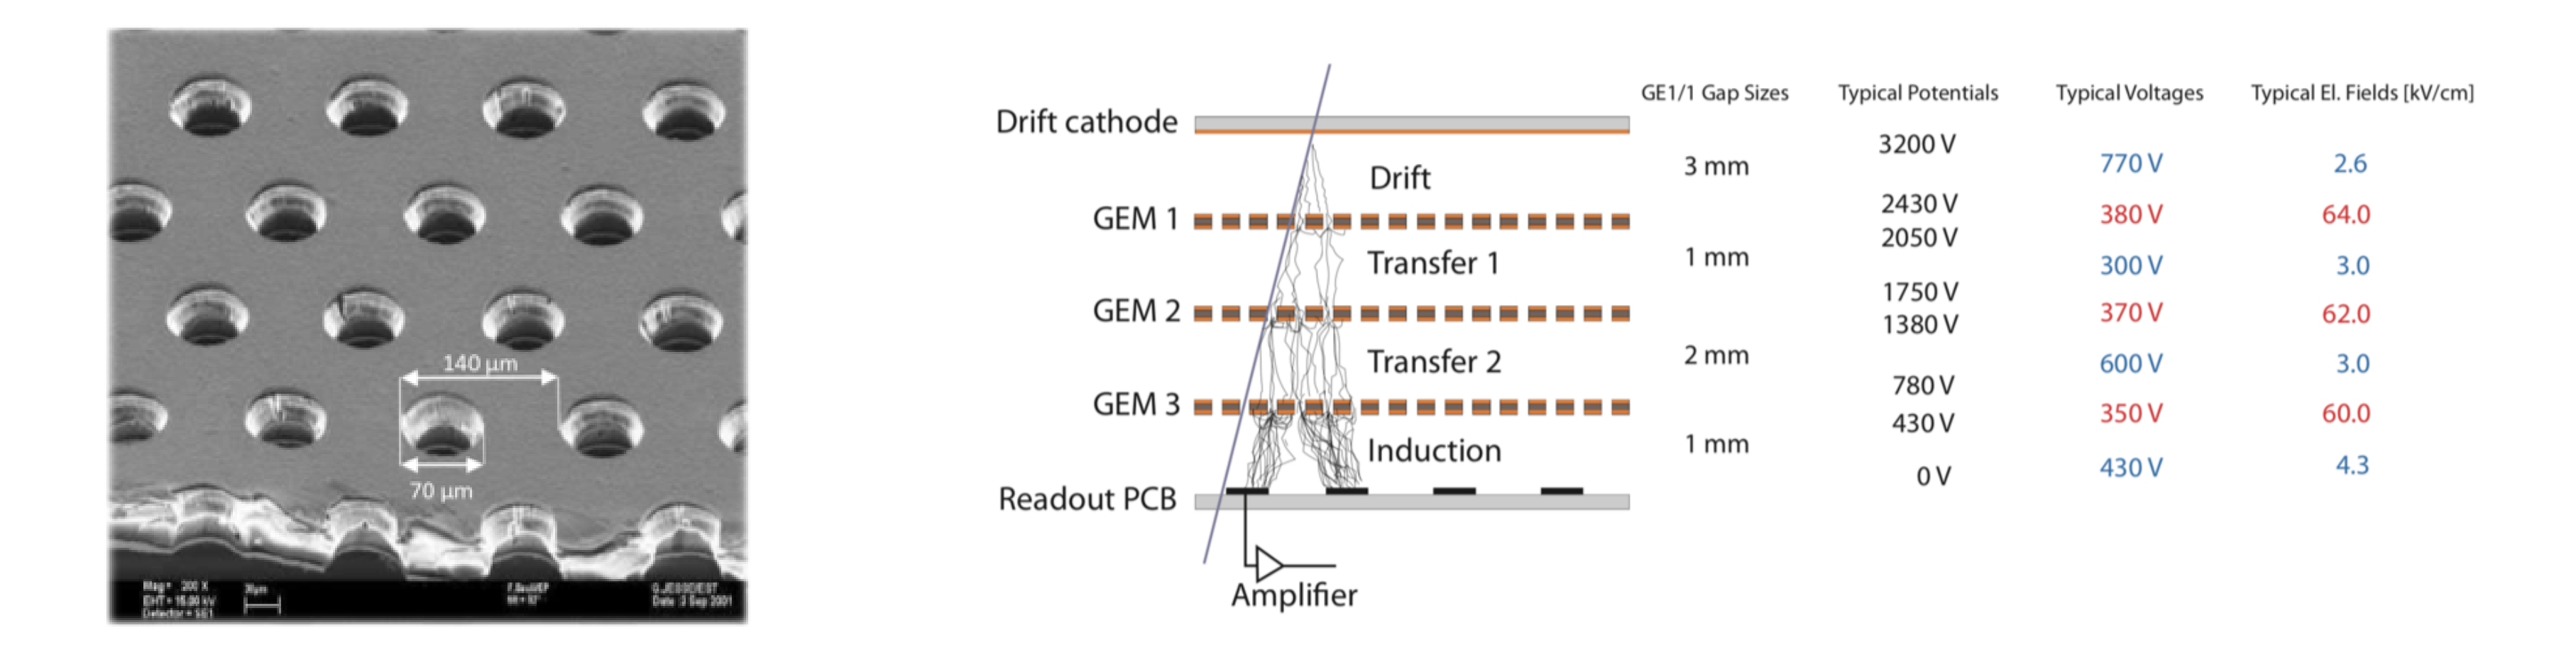
\includegraphics[width=\textwidth]{Images/CMS/GEMDiagram2.png}
    \caption{Left: a photograph of the micron-scale holes in the GEM foil. Right: The typical voltages in each layer of a GEM chamber.}
    \label{fig:GEMDiagram2}
\end{figure} 

\subsection{Trigger system} \label{sec:Trigger}

At the LHC's design luminosity, bunch crossings occur every \SI{25}{ns}. Most of these collisions result in low-energy multi-jet events with little potential for new physics searches. More rare are interesting physics events with smaller cross-sections (e.g., single- and pair-production of heavy bosons, top-antitop creation, digamma events, etc.), however, offline storage capacity limits the fraction of these events that can be kept. This requires CMS to include a fast trigger system \cite{Trigger} to identify events of potential interest with clean, high-quality particle signatures. The CMS trigger system is two-tiered: a low-level trigger built from custom-designed electronics and a high-level trigger that runs reconstruction and selection algorithms on comercial PCs.

\subsubsection{Level one trigger} \label{sec:L1Trigger}

The CMS Level-1 (L1) trigger makes the initial event selection to reduce the \SI{40}{MHz} collision rate. Both the muon system and the calorimeters separately generate packets of coarse-grain spatial and kinematic information of particle-candiates called trigger primitives (TPs). The L1 muon trigger is segmented into three regional track finders: the barrel muon track finder (BMTF), the overlap muon track finder (OMTF), and the endcap muon track finder (EMTF). Each muon subdetector (CSCs, DTs, and RPCs) passes hit information in the form of TPs carrying position, direction, and timing information to the regional track finders. The track finders then  separately reconstruct muon tracks and send that information to the Global Muon Trigger (GMT) which eliminates any redundant tracks based off $p_T$ and quality. The L1 calorimeter trigger combines TPs carrying energy information from the ECAL, HCAL, and HF. In the EB, a five-by-five array of ECAL crystals are combined into a trigger tower (TT), whose transverse energy sum forms a single TP (similarly in the EE, where TTs may have 5-25 crystals). Trigger Concentrator Cards (TCCs) collect TPs from the ECAL and HCAL and form electron, photon, jet, and hadronically-decaying tau candidates before they are combined in the Global Calorimeter Trigger (GCT). Reconstructed L1 trigger objects form the GMT and GCT are merged in the Global Trigger (GT), where they are compared to a ``menu'' of up to 128 algorithms (refered to as ``seeds''). If an event satisfies the criteria of at least one seed, an L1 accept (L1A) is sent upstream to the subdetectors. Upon reciept of an L1A, TPs and all detector information from the data aquisition (DAQ) system---stored in the buffers of onboard electronics---are sent downstream to be processed by the high-level trigger. The latency of the L1 trigger is fixed at approximately \SI{4}{\micro s}, a requirement set by the collision rate and the buffer sizes of the different subsytems, and sustains an output rate of \SI{100}{kHz}. A flow chart of the L1 trigger system is shown in Fig.~\ref{fig:L1TriggerMap}.

\begin{figure}[H]
    \centering
    {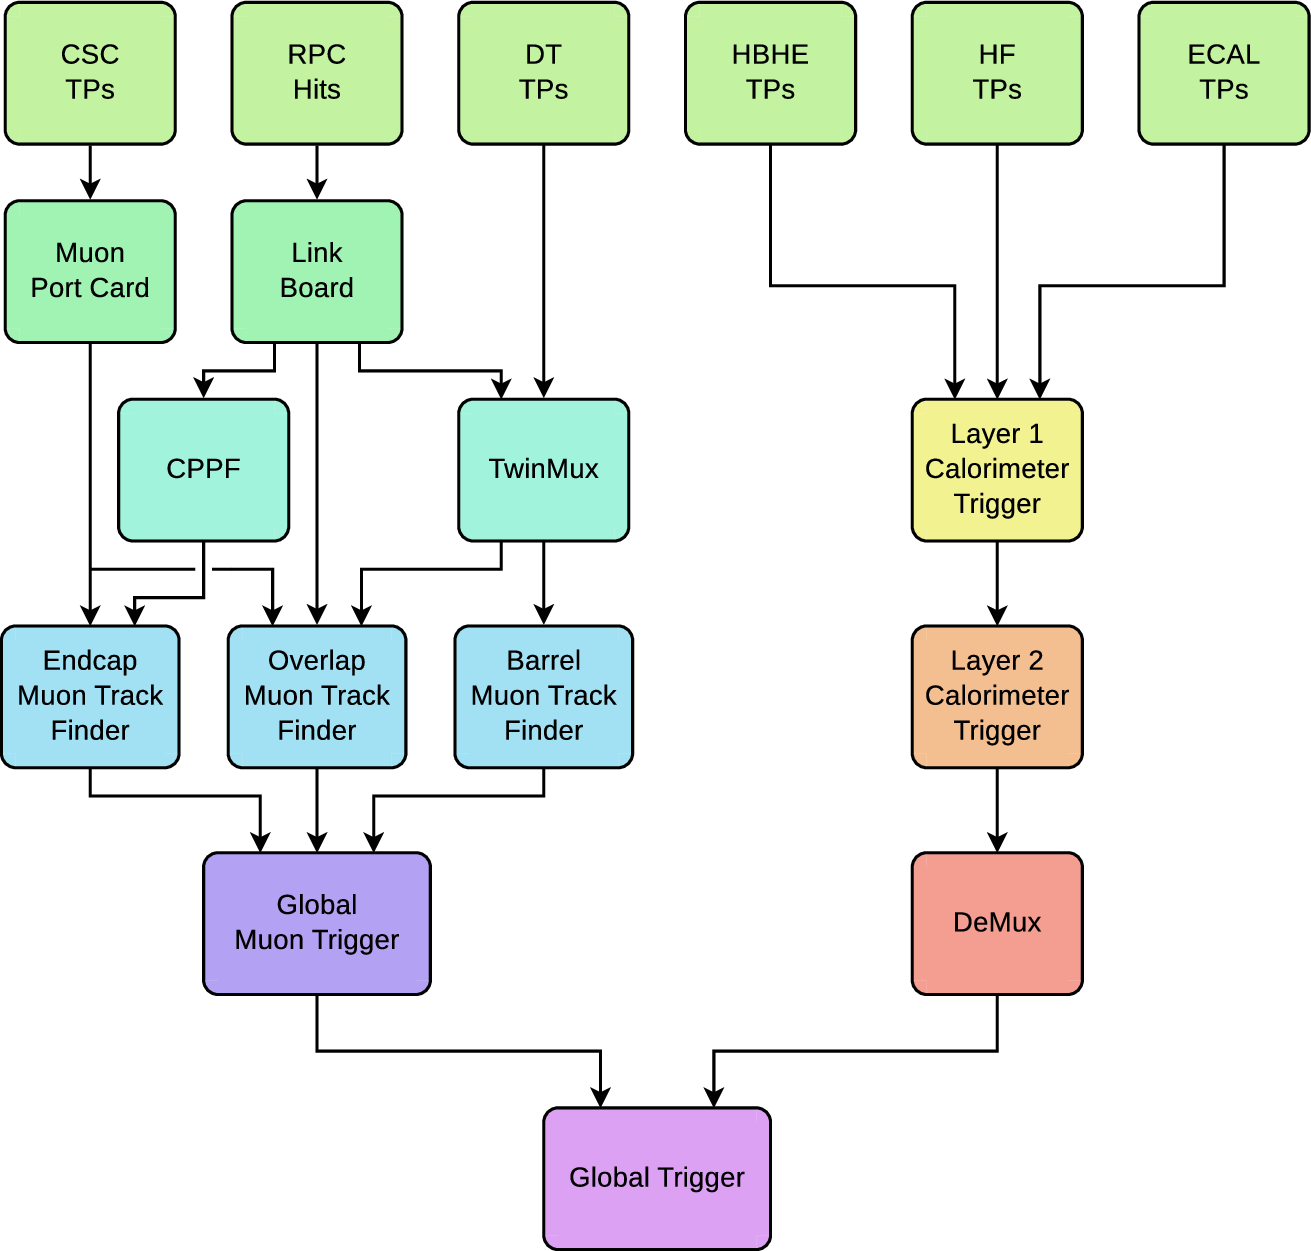
\includegraphics[width=\textwidth]{Images/CMS/L1TriggerMap.png}}
    \caption{A flow chart of the CMS L1 trigger system.}
    \label{fig:L1TriggerMap}
\end{figure}

\subsubsection{High-level trigger} \label{sec:HLT}
To further reduce the L1A output rate, the high-level trigger (HLT) makes a final selection of events with a \SI{1}{kHz} readout rate, acceptable for offline reconstruction and permanent storage. Implemented in software running on a farm of commercial computers, the HLT takes an L1A seed and performs a streamlined reconstruction with a similar efficiency to that used in offline processing. The HLT then filters events in roughly two stages: first, using only muon system and calorimeter information, and second, using full tracks. Events selected by the HLT algorithms are sent to permanent storage. A photograph of a GPU used to process the HLT algorithms is shown in Fig.~\ref{fig:HLTGPU}.

\begin{figure}[H]
    \centering
    {\includegraphics[width=\textwidth]{Images/CMS/HLTGPU.png}}
    \caption{A GPU used to process the HLT algorithms.}
    \label{fig:HLTGPU}
\end{figure} 